% Options for packages loaded elsewhere
\PassOptionsToPackage{unicode}{hyperref}
\PassOptionsToPackage{hyphens}{url}
\PassOptionsToPackage{dvipsnames,svgnames,x11names}{xcolor}
%
\documentclass[
  11pt,
]{krantz}
\usepackage{amsmath,amssymb}
\usepackage{lmodern}
\usepackage{iftex}
\ifPDFTeX
  \usepackage[T1]{fontenc}
  \usepackage[utf8]{inputenc}
  \usepackage{textcomp} % provide euro and other symbols
\else % if luatex or xetex
  \usepackage{unicode-math}
  \defaultfontfeatures{Scale=MatchLowercase}
  \defaultfontfeatures[\rmfamily]{Ligatures=TeX,Scale=1}
  \setmonofont[Scale=0.775]{MesloLGS NF}
\fi
% Use upquote if available, for straight quotes in verbatim environments
\IfFileExists{upquote.sty}{\usepackage{upquote}}{}
\IfFileExists{microtype.sty}{% use microtype if available
  \usepackage[]{microtype}
  \UseMicrotypeSet[protrusion]{basicmath} % disable protrusion for tt fonts
}{}
\makeatletter
\@ifundefined{KOMAClassName}{% if non-KOMA class
  \IfFileExists{parskip.sty}{%
    \usepackage{parskip}
  }{% else
    \setlength{\parindent}{0pt}
    \setlength{\parskip}{6pt plus 2pt minus 1pt}}
}{% if KOMA class
  \KOMAoptions{parskip=half}}
\makeatother
\usepackage{xcolor}
\IfFileExists{xurl.sty}{\usepackage{xurl}}{} % add URL line breaks if available
\IfFileExists{bookmark.sty}{\usepackage{bookmark}}{\usepackage{hyperref}}
\hypersetup{
  pdftitle={Appunti di Costruzione e validazione di strumenti di misura dell'efficacia dell'intervento psicologico in neuropsicologia -- B020881 (B213)},
  pdfauthor={Corrado Caudek},
  colorlinks=true,
  linkcolor={Maroon},
  filecolor={Maroon},
  citecolor={Blue},
  urlcolor={Blue},
  pdfcreator={LaTeX via pandoc}}
\urlstyle{same} % disable monospaced font for URLs
\usepackage{color}
\usepackage{fancyvrb}
\newcommand{\VerbBar}{|}
\newcommand{\VERB}{\Verb[commandchars=\\\{\}]}
\DefineVerbatimEnvironment{Highlighting}{Verbatim}{commandchars=\\\{\}}
% Add ',fontsize=\small' for more characters per line
\usepackage{framed}
\definecolor{shadecolor}{RGB}{248,248,248}
\newenvironment{Shaded}{\begin{snugshade}}{\end{snugshade}}
\newcommand{\AlertTok}[1]{\textcolor[rgb]{0.33,0.33,0.33}{#1}}
\newcommand{\AnnotationTok}[1]{\textcolor[rgb]{0.37,0.37,0.37}{\textbf{\textit{#1}}}}
\newcommand{\AttributeTok}[1]{\textcolor[rgb]{0.61,0.61,0.61}{#1}}
\newcommand{\BaseNTok}[1]{\textcolor[rgb]{0.06,0.06,0.06}{#1}}
\newcommand{\BuiltInTok}[1]{#1}
\newcommand{\CharTok}[1]{\textcolor[rgb]{0.5,0.5,0.5}{#1}}
\newcommand{\CommentTok}[1]{\textcolor[rgb]{0.37,0.37,0.37}{\textit{#1}}}
\newcommand{\CommentVarTok}[1]{\textcolor[rgb]{0.37,0.37,0.37}{\textbf{\textit{#1}}}}
\newcommand{\ConstantTok}[1]{\textcolor[rgb]{0,0,0}{#1}}
\newcommand{\ControlFlowTok}[1]{\textcolor[rgb]{0.27,0.27,0.27}{\textbf{#1}}}
\newcommand{\DataTypeTok}[1]{\textcolor[rgb]{0.27,0.27,0.27}{#1}}
\newcommand{\DecValTok}[1]{\textcolor[rgb]{0.06,0.06,0.06}{#1}}
\newcommand{\DocumentationTok}[1]{\textcolor[rgb]{0.37,0.37,0.37}{\textbf{\textit{#1}}}}
\newcommand{\ErrorTok}[1]{\textcolor[rgb]{0.14,0.14,0.14}{\textbf{#1}}}
\newcommand{\ExtensionTok}[1]{#1}
\newcommand{\FloatTok}[1]{\textcolor[rgb]{0.06,0.06,0.06}{#1}}
\newcommand{\FunctionTok}[1]{\textcolor[rgb]{0,0,0}{#1}}
\newcommand{\ImportTok}[1]{#1}
\newcommand{\InformationTok}[1]{\textcolor[rgb]{0.37,0.37,0.37}{\textbf{\textit{#1}}}}
\newcommand{\KeywordTok}[1]{\textcolor[rgb]{0.27,0.27,0.27}{\textbf{#1}}}
\newcommand{\NormalTok}[1]{#1}
\newcommand{\OperatorTok}[1]{\textcolor[rgb]{0.43,0.43,0.43}{\textbf{#1}}}
\newcommand{\OtherTok}[1]{\textcolor[rgb]{0.37,0.37,0.37}{#1}}
\newcommand{\PreprocessorTok}[1]{\textcolor[rgb]{0.37,0.37,0.37}{\textit{#1}}}
\newcommand{\RegionMarkerTok}[1]{#1}
\newcommand{\SpecialCharTok}[1]{\textcolor[rgb]{0,0,0}{#1}}
\newcommand{\SpecialStringTok}[1]{\textcolor[rgb]{0.5,0.5,0.5}{#1}}
\newcommand{\StringTok}[1]{\textcolor[rgb]{0.5,0.5,0.5}{#1}}
\newcommand{\VariableTok}[1]{\textcolor[rgb]{0,0,0}{#1}}
\newcommand{\VerbatimStringTok}[1]{\textcolor[rgb]{0.5,0.5,0.5}{#1}}
\newcommand{\WarningTok}[1]{\textcolor[rgb]{0.37,0.37,0.37}{\textbf{\textit{#1}}}}
\usepackage{longtable,booktabs,array}
\usepackage{calc} % for calculating minipage widths
% Correct order of tables after \paragraph or \subparagraph
\usepackage{etoolbox}
\makeatletter
\patchcmd\longtable{\par}{\if@noskipsec\mbox{}\fi\par}{}{}
\makeatother
% Allow footnotes in longtable head/foot
\IfFileExists{footnotehyper.sty}{\usepackage{footnotehyper}}{\usepackage{footnote}}
\makesavenoteenv{longtable}
\usepackage{graphicx}
\makeatletter
\def\maxwidth{\ifdim\Gin@nat@width>\linewidth\linewidth\else\Gin@nat@width\fi}
\def\maxheight{\ifdim\Gin@nat@height>\textheight\textheight\else\Gin@nat@height\fi}
\makeatother
% Scale images if necessary, so that they will not overflow the page
% margins by default, and it is still possible to overwrite the defaults
% using explicit options in \includegraphics[width, height, ...]{}
\setkeys{Gin}{width=\maxwidth,height=\maxheight,keepaspectratio}
% Set default figure placement to htbp
\makeatletter
\def\fps@figure{htbp}
\makeatother
\setlength{\emergencystretch}{3em} % prevent overfull lines
\providecommand{\tightlist}{%
  \setlength{\itemsep}{0pt}\setlength{\parskip}{0pt}}
\setcounter{secnumdepth}{5}
\usepackage{amsmath}
\usepackage{amssymb}
\usepackage{amsfonts}

\defaultfontfeatures{Scale=MatchLowercase}

\usepackage{booktabs}
\usepackage{longtable}
\usepackage[bf,singlelinecheck=off]{caption}

\usepackage{framed,color}
\definecolor{shadecolor}{RGB}{248,248,248}

\renewcommand{\textfraction}{0.05}
\renewcommand{\topfraction}{0.8}
\renewcommand{\bottomfraction}{0.8}
\renewcommand{\floatpagefraction}{0.75}

\renewenvironment{quote}{\begin{VF}}{\end{VF}}
\let\oldhref\href
\renewcommand{\href}[2]{#2\footnote{\url{#1}}}

\ifxetex
  \usepackage{letltxmacro}
  \setlength{\XeTeXLinkMargin}{1pt}
  \LetLtxMacro\SavedIncludeGraphics\includegraphics
  \def\includegraphics#1#{% #1 catches optional stuff (star/opt. arg.)
    \IncludeGraphicsAux{#1}%
  }%
  \newcommand*{\IncludeGraphicsAux}[2]{%
    \XeTeXLinkBox{%
      \SavedIncludeGraphics#1{#2}%
    }%
  }%
\fi

\makeatletter
\newenvironment{kframe}{%
\medskip{}
\setlength{\fboxsep}{.8em}
 \def\at@end@of@kframe{}%
 \ifinner\ifhmode%
  \def\at@end@of@kframe{\end{minipage}}%
  \begin{minipage}{\columnwidth}%
 \fi\fi%
 \def\FrameCommand##1{\hskip\@totalleftmargin \hskip-\fboxsep
 \colorbox{shadecolor}{##1}\hskip-\fboxsep
     % There is no \\@totalrightmargin, so:
     \hskip-\linewidth \hskip-\@totalleftmargin \hskip\columnwidth}%
 \MakeFramed {\advance\hsize-\width
   \@totalleftmargin\z@ \linewidth\hsize
   \@setminipage}}%
 {\par\unskip\endMakeFramed%
 \at@end@of@kframe}
\makeatother

\renewenvironment{Shaded}{\begin{kframe}}{\end{kframe}}

\usepackage{makeidx}
\makeindex

\urlstyle{tt}

\usepackage{amsthm}
\makeatletter
\def\thm@space@setup{%
  \thm@preskip=8pt plus 2pt minus 4pt
  \thm@postskip=\thm@preskip
}
\makeatother

\DeclareMathOperator{\V}{\mathbb{V}} % Define variance operator
\DeclareMathOperator{\Var}{\mathbb{V}} % Define variance operator
\DeclareMathOperator{\SD}{SD} % Define sd operator
\DeclareMathOperator{\Cov}{Cov} % Define covariance operator
\DeclareMathOperator{\Corr}{Corr} % Define correlation operator
\DeclareMathOperator{\Me}{Me} % Define mediane operator
\DeclareMathOperator{\Mo}{Mo} % Define mode operator

\DeclareMathOperator{\Bin}{Binomial} % Define binomial operator
\DeclareMathOperator{\Bernoulli}{Bernoulli} % Define Bernoulli operator
\DeclareMathOperator{\Ber}{\mathscr{B}} % Define Bernoulli operator
\DeclareMathOperator{\Poi}{Poisson} % Define Poisson operator
\DeclareMathOperator{\Uniform}{Uniform} % Define Uniform operator
\DeclareMathOperator{\Cauchy}{Cauchy} % Define Cauchy operator
\DeclareMathOperator{\B}{B} % beta function
% \mbox{B}(a, b) % beta function
% \mbox{Beta}(a, b) % beta distribution

\DeclareMathOperator{\elpd}{elpd} % Define elpd operator
\DeclareMathOperator{\lppd}{lppd} % Define lppd operator
\DeclareMathOperator{\LOO}{LOO} % Define LOO operator
\DeclareMathOperator{\argmin}{arg\,min} 
\DeclareMathOperator{\argmax}{arg\,max} 

\newcommand{\E}{\mathbb{E}} % Define expected value operator
\newcommand{\R}{\textsf{R}} % Define R programming language symbol
\newcommand{\Real}{\mathbb{R}} % Define real number operator
\newcommand{\Prob}{\mathscr{P}}
\newcommand{\indep}{\perp \!\!\! \perp}

\usepackage[
 labelfont=bf,
 font={small, it}
]{caption}
\usepackage{upquote} % print correct quotes in verbatim-environments
\usepackage{empheq}
\usepackage{xfrac}

\usepackage{polyglossia}
\setmainlanguage{italian}

\frontmatter
\ifLuaTeX
  \usepackage{selnolig}  % disable illegal ligatures
\fi
\usepackage[]{natbib}
\bibliographystyle{apalike}

\title{Appunti di Costruzione e validazione di strumenti di misura dell'efficacia dell'intervento psicologico in neuropsicologia -- B020881 (B213)}
\author{Corrado Caudek}
\date{2022-03-02}

\usepackage{amsthm}
\newtheorem{theorem}{Teorema}[chapter]
\newtheorem{lemma}{Lemma}[chapter]
\newtheorem{corollary}{Corollario}[chapter]
\newtheorem{proposition}{Proposizione}[chapter]
\newtheorem{conjecture}{Congettura}[chapter]
\theoremstyle{definition}
\newtheorem{definition}{Definizione}[chapter]
\theoremstyle{definition}
\newtheorem{example}{Esempio}[chapter]
\theoremstyle{definition}
\newtheorem{exercise}{Esercizio}[chapter]
\theoremstyle{definition}
\newtheorem{hypothesis}{Hypothesis}[chapter]
\theoremstyle{remark}
\newtheorem*{remark}{Osservazione}
\newtheorem*{solution}{Soluzione}
\begin{document}
\maketitle

\cleardoublepage\newpage\thispagestyle{empty}\null
% \cleardoublepage\newpage\thispagestyle{empty}\null
%\cleardoublepage\newpage
\thispagestyle{empty}
\begin{center}
\Large{Appunti di Costruzione e validazione di strumenti di misura dell'efficacia dell'intervento psicologico in neuropsicologia -- AA 2021/2022}

\vskip20pt

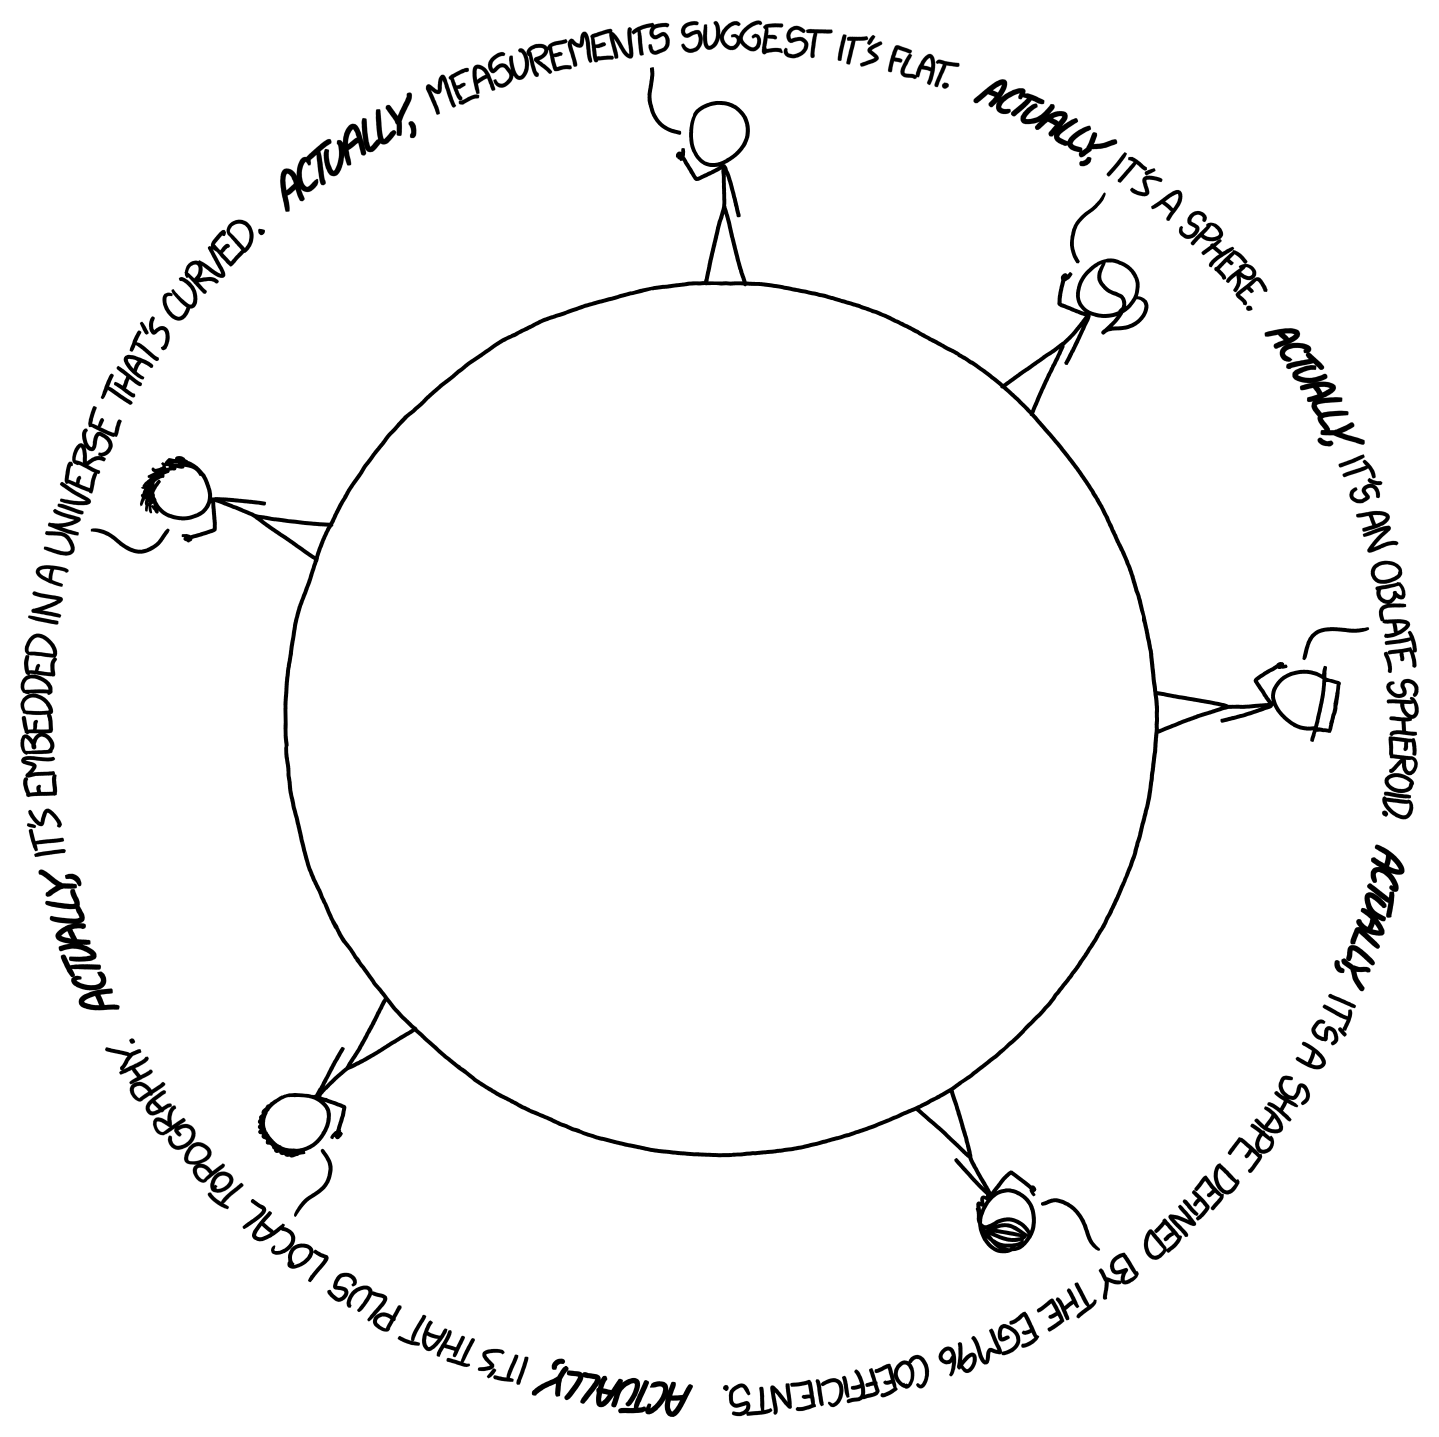
\includegraphics{images/actually_2x.png}
\end{center}

\setlength{\abovedisplayskip}{-5pt}
\setlength{\abovedisplayshortskip}{-5pt}

{
\hypersetup{linkcolor=}
\setcounter{tocdepth}{2}
\tableofcontents
}
\listoffigures
\listoftables
\hypertarget{prefazione}{%
\chapter*{Prefazione}\label{prefazione}}


La presente dispensa contiene il materiale delle lezioni dell'insegnamento di \emph{Costruzione e validazione di strumenti di misura dell'efficacia dell'intervento psicologico in neuropsicologia} B020881 (B213) rivolto agli studenti del secondo anno del Corso di Laurea Magistrale in Psicologia Clinica e della Salute e Neuropsicologia (curriculum: assessment e intervento psicologici in neuropsicologia - E21), A.A. 2021-2022. L'insegnamento si propone di fornire agli studenti un'introduzione all'assessment psicologico, ovvero un insieme di conoscenze/competenze che si pongono all'intersezione tra psicometria, statistica e informatica.

Nello specifico, l'insegnamento si focalizzerà sull'analisi fattoriale confermativa (\emph{confermatory factor analysis}, CFA) e sull'analisi fattoriale esplorativa, (\emph{explorative factor analysis}, EFA), cioè sugli strumenti che vengono usati durante il processo di sviluppo dei test psicometrici, ovvero che vengono usati per esaminare la struttura latente di una scala psicologica (ad esempio un questionario). In questo contesto, la CFA viene utilizzata per verificare il numero di dimensioni sottostanti gli indicatori (fattori) e l'intensità delle relazioni item-fattore (saturazioni fattoriali). La CFA consente anche di capire di come dovrebbe essere svolto lo scoring di un test. Quando la struttura latente è multifattoriale (cioè, a due o più fattori), il numero di fattori è indicativo del numero di sottoscale e di come esse dovrebbero essere codificate. La CFA è un importante strumento analitico anche per altri aspetti della valutazione psicometrica. Può essere utilizzata per stimare l'affidabilità di scala dei test psicometrici in modo da evitare i problemi della teoria classica dei test (ad es. alpha di Cronbach). Dati i recenti progressi nell'analisi dei dati categoriali, ora la CFA offre un quadro analitico comparabile a quello offerto dalla teoria di risposta agli item (IRT). In effetti, secondo \citet{brown2015confirmatory}, la CFA offre una maggiore flessibilità analitica rispetto al modello IRT tradizionale.

Un costrutto è un concetto teorico che può essere operazionalizzato nei termini di un fattore. In psicologia clinica, psichiatria e neuropsicologia, ad esempio, i disturbi mentali sono costrutti manifestati da vari insiemi di sintomi che sono riportati dal paziente o osservati da altri. La CFA è uno strumento analitico indispensabile per la validazione dei costrutti psicologici. I risultati della CFA possono fornire prove convincenti della validità convergente e discriminante dei costrutti teorici. La validità convergente è indicata dall'evidenza che diversi indicatori di costrutti teoricamente simili o sovrapposti sono fortemente correlati. La validità discriminante è indicata dai risultati che mostrano che gli indicatori di costrutti teoricamente distinti sono altamente incorrelati. Un punto di forza fondamentale degli approcci CFA per la costruzione e la validazione di uno strumento psicometrico è che le risultanti stime di validità convergente e discriminante sono corrette per l'errore di misurazione. Pertanto, la CFA fornisce un quadro analitico migliore rispetto ai metodi tradizionali che non tengono conto dell'errore di misurazione (ad esempio, gli approcci ordinari ai minimi quadrati come la correlazione/regressione multipla, i quali presuppongono che le variabili nell'analisi siano prive di errori di misurazione).

Spesso, parte della covariazione delle misure osservate è dovuta a fonti diverse dai fattori latenti di interesse. Questa covariazione aggiuntiva spesso riflette la varianza del metodo utilizzato per la misurazione. Gli effetti del metodo possono verificarsi anche all'interno di un'unica modalità di valutazione. Ad esempio, effetti del metodo sono solitamente presenti nei questionari che contengono una combinazione di elementi formulati positivamente e negativamente. Sfortunatamente, l'EFA non è in grado di stimare gli effetti del metodo. In effetti, l'uso di EFA quando esistono effetti del metodo può produrre risultati fuorvianti, ovvero suggerire la presenza di fattori aggiuntivi che corrispondono invece ad artefatti della misurazione. Nella CFA, invece, gli effetti del metodo possono essere specificati come parte della teoria dell'errore del modello di misurazione.

Un altro punto di forza della CFA è la sua capacità di affrontare il problema della generalizzabilità del modello di misurazione tra gruppi di individui o nel tempo. La valutazione dell'invarianza della misura è un aspetto importante dello sviluppo del test. Se un test è destinato a essere somministrato in una popolazione eterogenea, si dovrebbe stabilire che le sue proprietà di misurazione sono equivalenti in sottogruppi della popolazione (es. sesso, razza). Si dice che un test è distorto quando alcuni dei suoi elementi non misurano il costrutto sottostante in modo comparabile tra gruppi di rispondenti. Il test fornisce una stima distorta se, ad esempio, per un dato livello di vera intelligenza, gli uomini tendono a ottenere un punteggio di QI più alto rispetto alle donne. Il problema della generalizzabilità della validità del costrutto tra i gruppi può essere affrontato nella CFA esaminando gruppi multipli mediante modelli MIMIC (indicatori multipli, cause multiple). Inotre, è possibile chiedersi se il modello di misurazione sia equivalente tra i gruppi. Le soluzioni CFA a gruppi multipli vengono anche utilizzate per esaminare l'invarianza della misurazione longitudinale. Questo è un aspetto molto importante dell'analisi delle variabili latenti dei progetti di misure ripetute. In assenza di tale valutazione, non è possibile determinare se il cambiamento temporale in un costrutto sia dovuto a un vero cambiamento dei rispondenti o a cambiamenti nel modo di rispondere alla scala nel tempo. L'analisi a gruppi multipli può essere applicata a qualsiasi tipo di modello CFA. Ad esempio, queste procedure possono essere incorporate nell'analisi dei dati multitratto-multimetodo per esaminare la generalizzabilità della validità del costrutto tra gruppi.

In questo insegnamento la discussione delle teciche della CFA sarà preceduta da un'introduzione relativa alla EFA e la teoria classica dei test. La EFA, infatti, può essere concepita il metodo che viene utilizzato nei primi passi dello sviluppo di una scala psicometria, mentre la teoria classica dei test rappresenta la cornice teorica di partenza, di cui la CFA e i modelli di equazioni strutturali costituiscono uno sviluppo.

L'insegnamento pone una grande enfasi non solo sulla comprensione dei concetti teorici necessari per la costruzione e la validazione di uno strumento di misura in psicologia, ma anche sulla capacità di applicare tali concetti in situazioni concrete. Di conseguenza, la discussione dei concetti sarà sempre accompagnata da applicazioni pratiche. Tali applicazioni richiedono l'uso di un software. In questo insegnamento useremo \(\textsf{R}\) \citep{rmanual} quale linguaggio di programmazione probabilistica e, tra gli altri, il pacchetto \texttt{lavaan} che consente di svolgere le analisi statistiche della CFA e della EFA \citep{beaujean2014latent}. La teoria classica dei test verrà descritta con riferimento al classico testo di \citet{lord1968statistical}. Questa dispensa, inoltre, segue da vicino la trattazione della CFA fornita nei testi di \citet{mcdonald2013test} e di \citet{brown2015confirmatory}.

Trattando di argomenti avanzati, questo insegnamento presuppone la conoscenza di base dei concetti fondamentali della teoria delle probabilità; presuppone inoltre il possesso delle conoscenze di base necessarie per procedere all'utilizzo di \(\textsf{R}\). Informazioni su tali argomenti sono forniti nella dispensa di Psicometria (A.A. 2021-2022).

\begin{flushright}
Corrado Caudek\\
Marzo 2022 \end{flushright}

\mainmatter

\hypertarget{part-il-modello-lineare}{%
\part{Il modello lineare}\label{part-il-modello-lineare}}

\hypertarget{lanalisi-di-regressione}{%
\chapter{L'analisi di regressione}\label{lanalisi-di-regressione}}

Conoscere l'analisi di regressione aiuta a capire la teoria classica dei test, l'analisi fattoriale e i modelli di equazioni strutturali. Sebbene le tecniche dell'analisi di regressione analizzino solo le variabili osservate, i principi della regressione costituiscono la base delle tecniche più avanzate che includono anche le variabili latenti.

\hypertarget{regressione-bivariata}{%
\section{Regressione bivariata}\label{regressione-bivariata}}

Il modello di regressione bivariata descrive l'associazione tra il valore atteso di \(Y \mid x_i\) e \(x\) nei termini di una relazione lineare:

\[
\mathbb{E}(Y \mid x_i) = \alpha + \beta x_i,
\] dove i valori \(x_i\) sono considerati fissi per disegno. Nel modello ``classico'', si assume che le distribuzioni \(Y \mid x_i\) siano Normali con deviazione standard \(\sigma_\varepsilon\).

Il significato dei coefficienti di regressione è semplice:

\begin{itemize}
\tightlist
\item
  \(\alpha\) è il valore atteso di \(Y\) quando \(X = 0\);
\item
  \(\beta\) è l'incremento atteso nel valore atteso di \(Y\) quando \(X\) aumenta di un'unità.
\end{itemize}

Per fare un esempio, consideriamo i dati dell'antropologo Sahlins, il quale si è chiesto se esiste un'associazione tra l'ampiezza del clan (\texttt{consumers}) e l'area occupata da quel clan (\texttt{acres}) in una popolazione di cacciatori-raccoglitori. I dati sono i seguenti:

\begin{Shaded}
\begin{Highlighting}[]
\FunctionTok{data}\NormalTok{(Sahlins)}
\FunctionTok{head}\NormalTok{(Sahlins)}
\CommentTok{\#\textgreater{}   consumers acres}
\CommentTok{\#\textgreater{} 1      1.00  1.71}
\CommentTok{\#\textgreater{} 2      1.08  1.52}
\CommentTok{\#\textgreater{} 3      1.15  1.29}
\CommentTok{\#\textgreater{} 4      1.15  3.09}
\CommentTok{\#\textgreater{} 5      1.20  2.21}
\CommentTok{\#\textgreater{} 6      1.30  2.26}
\end{Highlighting}
\end{Shaded}

\begin{Shaded}
\begin{Highlighting}[]
\NormalTok{Sahlins }\SpecialCharTok{\%\textgreater{}\%}
  \FunctionTok{ggplot}\NormalTok{(}\FunctionTok{aes}\NormalTok{(}\AttributeTok{x =}\NormalTok{ consumers, }\AttributeTok{y =}\NormalTok{ acres)) }\SpecialCharTok{+}
  \FunctionTok{geom\_point}\NormalTok{() }\SpecialCharTok{+}
  \FunctionTok{geom\_smooth}\NormalTok{(}\AttributeTok{method =}\NormalTok{ lm, }\AttributeTok{se =} \ConstantTok{FALSE}\NormalTok{)}
\end{Highlighting}
\end{Shaded}

\begin{center}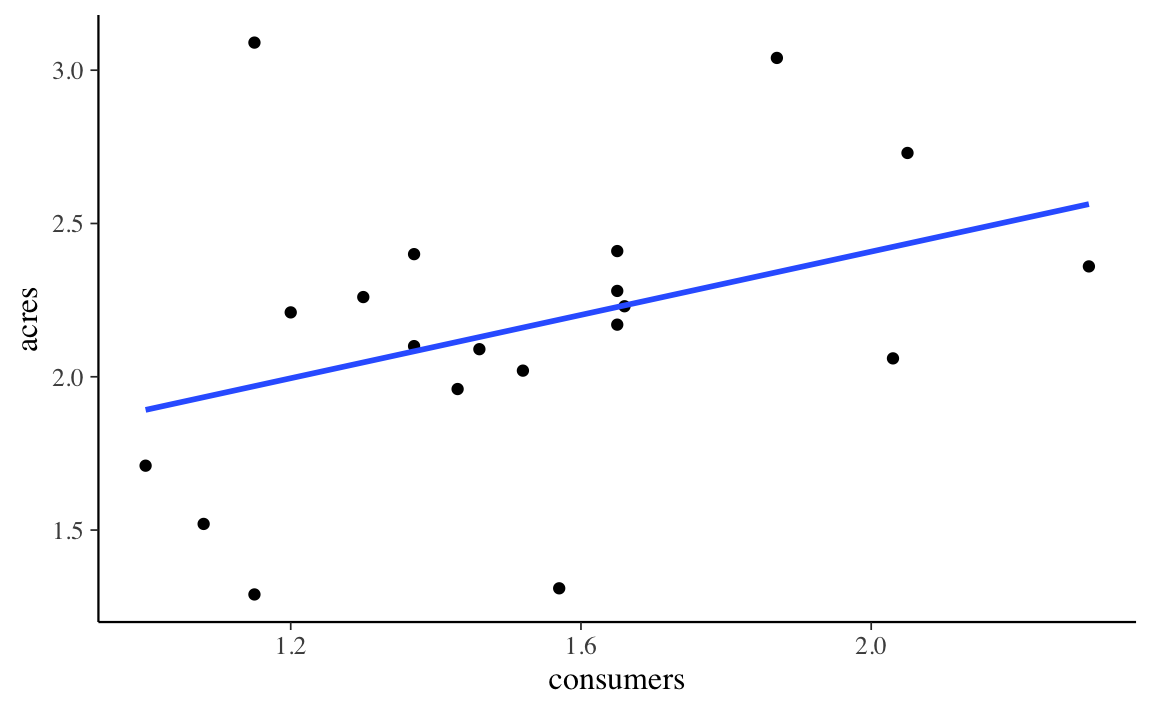
\includegraphics{cfa_book_files/figure-latex/unnamed-chunk-4-1} \end{center}

\begin{Shaded}
\begin{Highlighting}[]
\NormalTok{fm }\OtherTok{\textless{}{-}} \FunctionTok{lm}\NormalTok{(acres }\SpecialCharTok{\textasciitilde{}}\NormalTok{ consumers, }\AttributeTok{data =}\NormalTok{ Sahlins)}
\NormalTok{fm}\SpecialCharTok{$}\NormalTok{coef}
\CommentTok{\#\textgreater{} (Intercept)   consumers }
\CommentTok{\#\textgreater{}      1.3756      0.5163}
\end{Highlighting}
\end{Shaded}

Dalla figura notiamo che, se \texttt{consumers} aumenta di un'unità (da 1.2 a 2.2), allora la retta di regressione (ovvero, il valore atteso di \(Y\)) aumenta di circa 0.5 punti -- esattamente, aumenta di 0.5163 punti, come indicato dalla stima del coefficiente \(\beta\). L'interpretazione del coefficiente \(\alpha\) è più problematica, perché non ha senso pensare ad un clan di ampiezza 0. Per affrontare questo problema, centriamo il predittore.

\hypertarget{regressori-centrati}{%
\subsection{Regressori centrati}\label{regressori-centrati}}

Esprimiamo la variabile \texttt{consumers} nei termini degli scarti dalla media:

\begin{Shaded}
\begin{Highlighting}[]
\NormalTok{Sahlins }\OtherTok{\textless{}{-}}\NormalTok{ Sahlins }\SpecialCharTok{\%\textgreater{}\%}
  \FunctionTok{mutate}\NormalTok{(}
    \AttributeTok{xc =}\NormalTok{ consumers }\SpecialCharTok{{-}} \FunctionTok{mean}\NormalTok{(consumers)}
\NormalTok{  )}
\end{Highlighting}
\end{Shaded}

Svolgiamo nuovamente l'analisi di regressione con il nuovo predittore:

\begin{Shaded}
\begin{Highlighting}[]
\NormalTok{fm1 }\OtherTok{\textless{}{-}} \FunctionTok{lm}\NormalTok{(acres }\SpecialCharTok{\textasciitilde{}}\NormalTok{ xc, }\AttributeTok{data =}\NormalTok{ Sahlins)}
\NormalTok{fm1}\SpecialCharTok{$}\NormalTok{coef}
\CommentTok{\#\textgreater{} (Intercept)          xc }
\CommentTok{\#\textgreater{}      2.1620      0.5163}
\end{Highlighting}
\end{Shaded}

\begin{Shaded}
\begin{Highlighting}[]
\NormalTok{Sahlins }\SpecialCharTok{\%\textgreater{}\%}
  \FunctionTok{ggplot}\NormalTok{(}\FunctionTok{aes}\NormalTok{(}\AttributeTok{x =}\NormalTok{ xc, }\AttributeTok{y =}\NormalTok{ acres)) }\SpecialCharTok{+}
  \FunctionTok{geom\_point}\NormalTok{() }\SpecialCharTok{+}
  \FunctionTok{geom\_smooth}\NormalTok{(}\AttributeTok{method =}\NormalTok{ lm, }\AttributeTok{se =} \ConstantTok{FALSE}\NormalTok{)}
\end{Highlighting}
\end{Shaded}

\begin{center}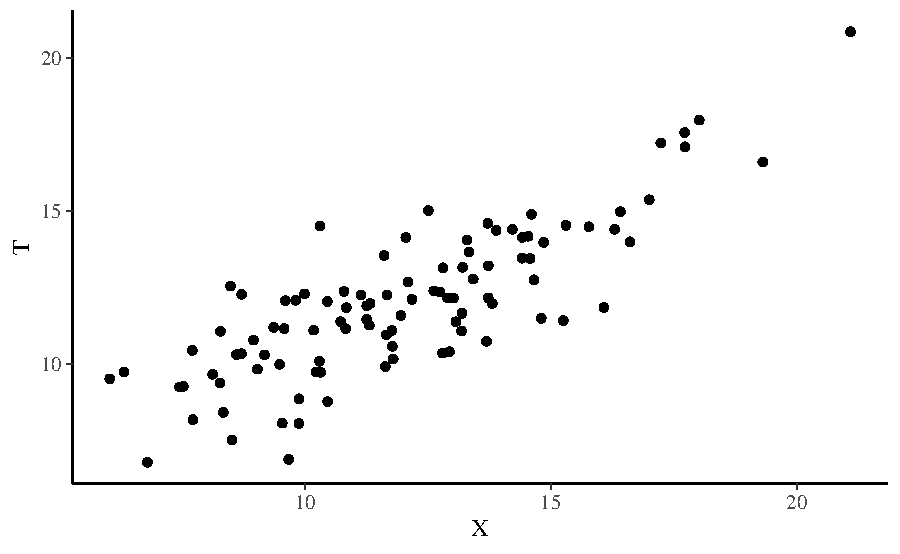
\includegraphics{cfa_book_files/figure-latex/unnamed-chunk-8-1} \end{center}

La stima di \(\beta\) è rimasta invariata ma ora possiamo attribuire un significato alla stima di \(\alpha\): questo coefficiente indica il valore atteso della \(Y\) quando \(X\) assume il suo valore medio.

\hypertarget{minimi-quadrati}{%
\subsection{Minimi quadrati}\label{minimi-quadrati}}

La stima dei coefficienti del modello di regressione può essere effettuata in modi diversi: massima verosimiglianza o metodi bayesiani. Se ci limitiamo qui alla massima verosimiglianza possiamo semplificare il problema assumento che le distribuzioni condizionate \(Y \mid x\) siano Normali. In tali circostanze, la stima dei coefficienti del modello di regressione può essere trovata con il metodo dei minimi quadrati.

In pratica, questo significa trovare i coefficienti \(a\) e \(b\) che minimizzano

\[
SS_{\text{res}} = \sum(y_i - \hat{y}_i)^2,
\] con \(\hat{y}_i = a + b x_i\).

Per fornire un'idea di come questo viene fatto, usiamo una simulazione. Per semplicità, supponiamo di conoscere \(a = 1.3756445\) e di volere stimare \(b\).

\begin{Shaded}
\begin{Highlighting}[]
\NormalTok{x }\OtherTok{\textless{}{-}}\NormalTok{ Sahlins}\SpecialCharTok{$}\NormalTok{consumers}
\NormalTok{y }\OtherTok{\textless{}{-}}\NormalTok{ Sahlins}\SpecialCharTok{$}\NormalTok{acres}
\NormalTok{a }\OtherTok{\textless{}{-}} \FloatTok{1.3756445}

\NormalTok{nrep }\OtherTok{\textless{}{-}} \FloatTok{1e3}
\NormalTok{b }\OtherTok{\textless{}{-}} \FunctionTok{seq}\NormalTok{(}\DecValTok{0}\NormalTok{, }\DecValTok{1}\NormalTok{, }\AttributeTok{length.out =}\NormalTok{ nrep)}

\NormalTok{ssres }\OtherTok{\textless{}{-}} \FunctionTok{rep}\NormalTok{(}\ConstantTok{NA}\NormalTok{, nrep)}
\ControlFlowTok{for}\NormalTok{ (i }\ControlFlowTok{in} \DecValTok{1}\SpecialCharTok{:}\NormalTok{nrep) \{}
\NormalTok{  yhat }\OtherTok{\textless{}{-}}\NormalTok{ a }\SpecialCharTok{+}\NormalTok{ b[i] }\SpecialCharTok{*}\NormalTok{ x}
\NormalTok{  ssres[i] }\OtherTok{\textless{}{-}} \FunctionTok{sum}\NormalTok{((y }\SpecialCharTok{{-}}\NormalTok{ yhat)}\SpecialCharTok{\^{}}\DecValTok{2}\NormalTok{)}
\NormalTok{\}}
\end{Highlighting}
\end{Shaded}

Un grafico di \(SS_{\text{res}}\) in funzione di \(b\) mostra che il valore \(b\) che minimizza \(SS_{\text{res}}\) corrisponde, appunto, a 0.5163.

\begin{Shaded}
\begin{Highlighting}[]
\FunctionTok{tibble}\NormalTok{(b, ssres) }\SpecialCharTok{\%\textgreater{}\%}
  \FunctionTok{ggplot}\NormalTok{(}\FunctionTok{aes}\NormalTok{(}\AttributeTok{x =}\NormalTok{ b, }\AttributeTok{y =}\NormalTok{ ssres)) }\SpecialCharTok{+}
  \FunctionTok{geom\_line}\NormalTok{()}
\end{Highlighting}
\end{Shaded}

\begin{center}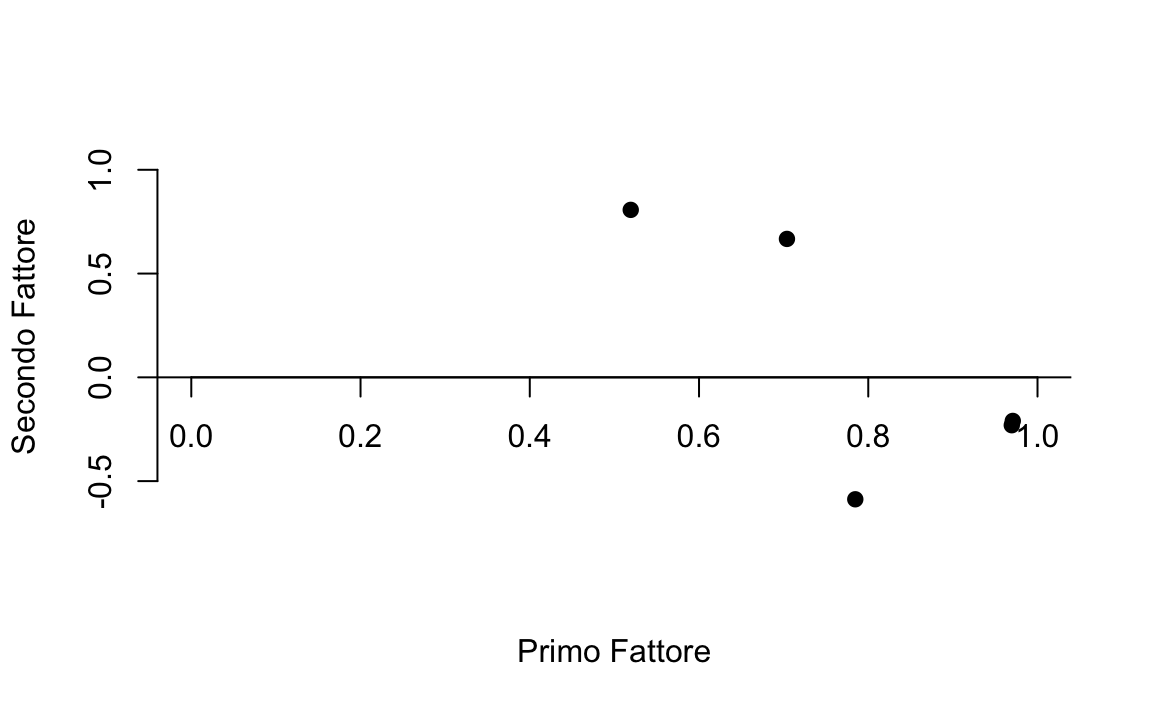
\includegraphics{cfa_book_files/figure-latex/unnamed-chunk-10-1} \end{center}

\hypertarget{relazione-tra-b-e-r}{%
\subsection{\texorpdfstring{Relazione tra \(b\) e \(r\)}{Relazione tra b e r}}\label{relazione-tra-b-e-r}}

Un altro modo per interpretare \(b\) è quello di considerare la relazione tra la pendenza della retta di regressione e il coefficiente di correlazione:

\[
b_X = r_{XY} \frac{S_X}{S_Y}
\]

L'equazione precedente rende chiaro che, se i dati sono standardizzati, \(b = r\).

Verifichiamo:

\begin{Shaded}
\begin{Highlighting}[]
\NormalTok{Sahlins }\SpecialCharTok{\%\textgreater{}\%}
\NormalTok{  dplyr}\SpecialCharTok{::}\FunctionTok{select}\NormalTok{(acres, consumers) }\SpecialCharTok{\%\textgreater{}\%}
  \FunctionTok{cor}\NormalTok{()}
\CommentTok{\#\textgreater{}            acres consumers}
\CommentTok{\#\textgreater{} acres     1.0000    0.3757}
\CommentTok{\#\textgreater{} consumers 0.3757    1.0000}
\end{Highlighting}
\end{Shaded}

\begin{Shaded}
\begin{Highlighting}[]
\NormalTok{fm2 }\OtherTok{\textless{}{-}} \FunctionTok{lm}\NormalTok{(}\FunctionTok{scale}\NormalTok{(acres) }\SpecialCharTok{\textasciitilde{}} \FunctionTok{scale}\NormalTok{(consumers), }\AttributeTok{data =}\NormalTok{ Sahlins)}
\NormalTok{fm2}\SpecialCharTok{$}\NormalTok{coef}
\CommentTok{\#\textgreater{}      (Intercept) scale(consumers) }
\CommentTok{\#\textgreater{}        9.917e{-}17        3.757e{-}01}
\end{Highlighting}
\end{Shaded}

\hypertarget{attenuazione}{%
\subsection{Attenuazione}\label{attenuazione}}

Il fenomeno dell'attenuazione si verifica quando \(X\) viene misurato con una componente di errore. Esaminiamo la seguente simulazione.

\begin{Shaded}
\begin{Highlighting}[]
\FunctionTok{set.seed}\NormalTok{(}\DecValTok{1234}\NormalTok{)}
\NormalTok{n }\OtherTok{\textless{}{-}} \DecValTok{100}
\NormalTok{x }\OtherTok{\textless{}{-}} \FunctionTok{rnorm}\NormalTok{(n, }\DecValTok{10}\NormalTok{, }\FloatTok{1.5}\NormalTok{)}
\NormalTok{y }\OtherTok{\textless{}{-}} \FloatTok{1.5} \SpecialCharTok{*}\NormalTok{ x }\SpecialCharTok{+} \FunctionTok{rnorm}\NormalTok{(n, }\DecValTok{0}\NormalTok{, }\DecValTok{2}\NormalTok{)}
\FunctionTok{tibble}\NormalTok{(x, y) }\SpecialCharTok{\%\textgreater{}\%}
  \FunctionTok{ggplot}\NormalTok{(}\FunctionTok{aes}\NormalTok{(x, y)) }\SpecialCharTok{+}
  \FunctionTok{geom\_point}\NormalTok{()}
\end{Highlighting}
\end{Shaded}

\begin{center}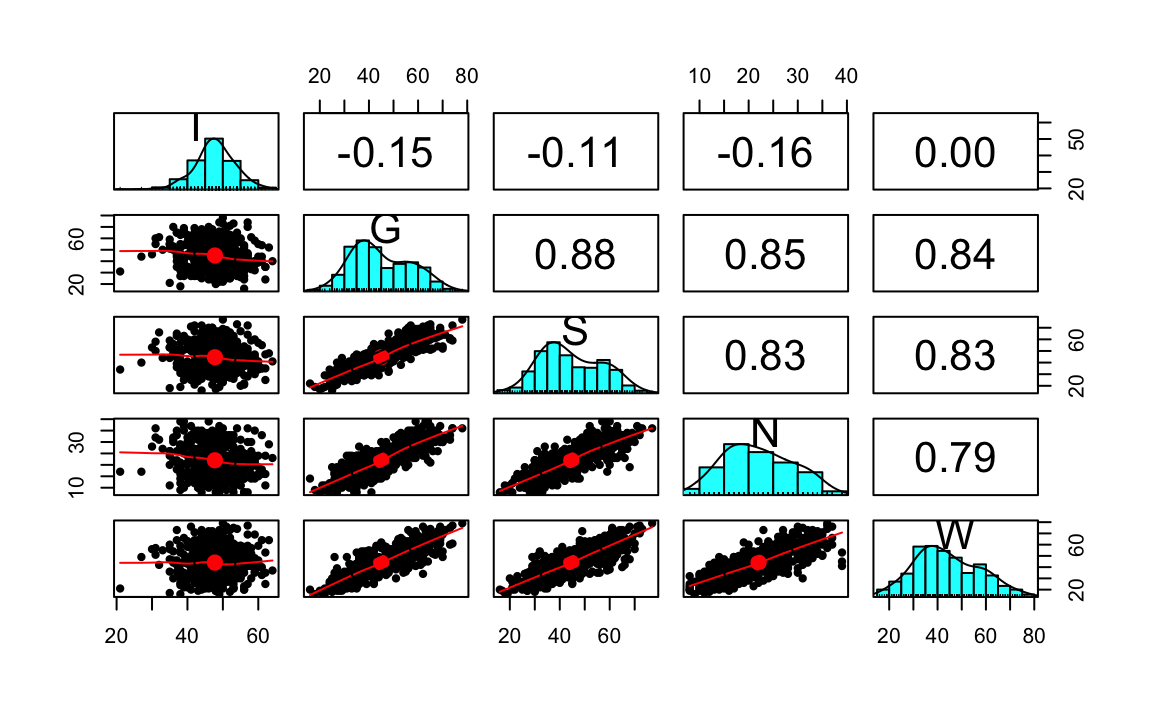
\includegraphics{cfa_book_files/figure-latex/unnamed-chunk-13-1} \end{center}

\begin{Shaded}
\begin{Highlighting}[]
\NormalTok{sim\_dat }\OtherTok{\textless{}{-}} \FunctionTok{tibble}\NormalTok{(x, y)}
\NormalTok{fm }\OtherTok{\textless{}{-}} \FunctionTok{lm}\NormalTok{(y }\SpecialCharTok{\textasciitilde{}}\NormalTok{ x, sim\_dat)}
\NormalTok{fm}\SpecialCharTok{$}\NormalTok{coef}
\CommentTok{\#\textgreater{} (Intercept)           x }
\CommentTok{\#\textgreater{}      0.4221      1.4652}
\end{Highlighting}
\end{Shaded}

Questi sono i coefficienti di regressione quando \(X\) è misurata senza errori.

\begin{Shaded}
\begin{Highlighting}[]
\NormalTok{sim\_dat }\OtherTok{\textless{}{-}}\NormalTok{ sim\_dat }\SpecialCharTok{\%\textgreater{}\%}
  \FunctionTok{mutate}\NormalTok{(}
    \AttributeTok{x1 =}\NormalTok{ x }\SpecialCharTok{+} \FunctionTok{rnorm}\NormalTok{(n, }\DecValTok{0}\NormalTok{, }\DecValTok{2}\NormalTok{)}
\NormalTok{  )}

\NormalTok{fm1 }\OtherTok{\textless{}{-}} \FunctionTok{lm}\NormalTok{(y }\SpecialCharTok{\textasciitilde{}}\NormalTok{ x1, sim\_dat)}
\NormalTok{fm1}\SpecialCharTok{$}\NormalTok{coef}
\CommentTok{\#\textgreater{} (Intercept)          x1 }
\CommentTok{\#\textgreater{}      8.3872      0.6296}
\end{Highlighting}
\end{Shaded}

Aggiungendo una componente d'errore su \(X\), la grandezza del coefficiente \(b\) diminuisce.

\hypertarget{coefficiente-di-determinazione}{%
\subsection{Coefficiente di determinazione}\label{coefficiente-di-determinazione}}

Tecnicamente, il coefficiente di determinazione è dato da:

\[
R^2 = \frac{\sum(\hat{y} - \bar{y})^2}{\sum(y_i - \bar{y})^2}
\]

Al denominatore abbiamo la \emph{devianza totale}, ovvero una misura della dispersione di \(y_i\) rispetto alla media \(\bar{y}\). Al numeratore abbiamo una misura della dispersione del valore atteso della \(Y\) rispetto alla sua media. Il rapporto, dunque, ci dice qual è la quota della variabilità totale di \(Y\) che può essere predetta in base al modello lineare.

Per i dati di Sahlins abbiamo:

\begin{Shaded}
\begin{Highlighting}[]
\NormalTok{mod }\OtherTok{\textless{}{-}} \FunctionTok{lm}\NormalTok{(acres }\SpecialCharTok{\textasciitilde{}}\NormalTok{ consumers, }\AttributeTok{data =}\NormalTok{ Sahlins)}
\NormalTok{a }\OtherTok{\textless{}{-}}\NormalTok{ mod}\SpecialCharTok{$}\NormalTok{coef[}\DecValTok{1}\NormalTok{]}
\NormalTok{b }\OtherTok{\textless{}{-}}\NormalTok{ mod}\SpecialCharTok{$}\NormalTok{coef[}\DecValTok{2}\NormalTok{]}
\NormalTok{yhat }\OtherTok{\textless{}{-}}\NormalTok{ a }\SpecialCharTok{+}\NormalTok{ b }\SpecialCharTok{*}\NormalTok{ Sahlins}\SpecialCharTok{$}\NormalTok{consumers}
\NormalTok{ss\_tot }\OtherTok{\textless{}{-}} \FunctionTok{sum}\NormalTok{((Sahlins}\SpecialCharTok{$}\NormalTok{acres }\SpecialCharTok{{-}} \FunctionTok{mean}\NormalTok{(Sahlins}\SpecialCharTok{$}\NormalTok{acres))}\SpecialCharTok{\^{}}\DecValTok{2}\NormalTok{)}
\NormalTok{ss\_reg }\OtherTok{\textless{}{-}} \FunctionTok{sum}\NormalTok{((yhat }\SpecialCharTok{{-}} \FunctionTok{mean}\NormalTok{(Sahlins}\SpecialCharTok{$}\NormalTok{acres))}\SpecialCharTok{\^{}}\DecValTok{2}\NormalTok{)}
\NormalTok{r2 }\OtherTok{\textless{}{-}}\NormalTok{ ss\_reg }\SpecialCharTok{/}\NormalTok{ ss\_tot}
\NormalTok{r2}
\CommentTok{\#\textgreater{} [1] 0.1411}
\end{Highlighting}
\end{Shaded}

Verifichiamo:

\begin{Shaded}
\begin{Highlighting}[]
\FunctionTok{summary}\NormalTok{(mod)}
\CommentTok{\#\textgreater{} }
\CommentTok{\#\textgreater{} Call:}
\CommentTok{\#\textgreater{} lm(formula = acres \textasciitilde{} consumers, data = Sahlins)}
\CommentTok{\#\textgreater{} }
\CommentTok{\#\textgreater{} Residuals:}
\CommentTok{\#\textgreater{}     Min      1Q  Median      3Q     Max }
\CommentTok{\#\textgreater{} {-}0.8763 {-}0.1873 {-}0.0211  0.2135  1.1206 }
\CommentTok{\#\textgreater{} }
\CommentTok{\#\textgreater{} Coefficients:}
\CommentTok{\#\textgreater{}             Estimate Std. Error t value Pr(\textgreater{}|t|)   }
\CommentTok{\#\textgreater{} (Intercept)    1.376      0.468    2.94   0.0088 **}
\CommentTok{\#\textgreater{} consumers      0.516      0.300    1.72   0.1026   }
\CommentTok{\#\textgreater{} {-}{-}{-}}
\CommentTok{\#\textgreater{} Signif. codes:  }
\CommentTok{\#\textgreater{} 0 \textquotesingle{}***\textquotesingle{} 0.001 \textquotesingle{}**\textquotesingle{} 0.01 \textquotesingle{}*\textquotesingle{} 0.05 \textquotesingle{}.\textquotesingle{} 0.1 \textquotesingle{} \textquotesingle{} 1}
\CommentTok{\#\textgreater{} }
\CommentTok{\#\textgreater{} Residual standard error: 0.454 on 18 degrees of freedom}
\CommentTok{\#\textgreater{} Multiple R{-}squared:  0.141,  Adjusted R{-}squared:  0.0934 }
\CommentTok{\#\textgreater{} F{-}statistic: 2.96 on 1 and 18 DF,  p{-}value: 0.103}
\end{Highlighting}
\end{Shaded}

Da cui deriva che \(R^2\) è uguale al quadrato del coefficiente di correlazione:

\begin{Shaded}
\begin{Highlighting}[]
\FunctionTok{cor}\NormalTok{(Sahlins}\SpecialCharTok{$}\NormalTok{acres, Sahlins}\SpecialCharTok{$}\NormalTok{consumers)}\SpecialCharTok{\^{}}\DecValTok{2}
\CommentTok{\#\textgreater{} [1] 0.1411}
\end{Highlighting}
\end{Shaded}

\hypertarget{errore-standard-della-regressione}{%
\subsection{Errore standard della regressione}\label{errore-standard-della-regressione}}

L'errore standard della regressione è una stima della dispersione di \(y \mid x_i\) nella popolazione. Non è altro che la deviazione standard dei residui

\[
e = y_i - \hat{y}_i
\]

che, al denominatore, riporta \(n-2\). La ragione è che, per calcolare \(\hat{y}\), vengono ``perduti'' due gradi di libertà -- il calcolo di \(\hat{y}\) è basato sulla stima di due coefficienti: \(a\) e \(b\).

\begin{Shaded}
\begin{Highlighting}[]
\NormalTok{e }\OtherTok{\textless{}{-}}\NormalTok{ yhat }\SpecialCharTok{{-}}\NormalTok{ Sahlins}\SpecialCharTok{$}\NormalTok{acres}
\NormalTok{(}\FunctionTok{sum}\NormalTok{(e}\SpecialCharTok{\^{}}\DecValTok{2}\NormalTok{) }\SpecialCharTok{/}\NormalTok{ (}\FunctionTok{length}\NormalTok{(Sahlins}\SpecialCharTok{$}\NormalTok{acres) }\SpecialCharTok{{-}} \DecValTok{2}\NormalTok{)) }\SpecialCharTok{\%\textgreater{}\%}
  \FunctionTok{sqrt}\NormalTok{()}
\CommentTok{\#\textgreater{} [1] 0.4543}
\end{Highlighting}
\end{Shaded}

Il valore trovato corrisponde a quello riportato nell'output di \texttt{lm()}.

\hypertarget{regressione-multipla}{%
\section{Regressione multipla}\label{regressione-multipla}}

Nella regressione multipla vengono utilizzati \(k > 1\) predittori:

\[
y_i = \alpha + \sum_{j=1}^k \beta_j x_i + \varepsilon_i.
\] L'interpretazione geometrica è simile a quella del modello bivariato. Nel caso di due predittori, il valore atteso della \(y\) può essere rappresentato da un piano; nel caso di \(k > 2\) predittori, da un iper-piano. Nel caso di \(k=2\), tale piano è posto in uno spazio di dimensioni \(x_1\), \(x_2\) (che possiamo immaginare definire un piano orizzontale) e \(y\) (ortogonale a tale piano). La superficie piana che rappresenta \(\mathbb{E}(y)\) è inclinata in maniera tale che l'angolo tra il piano e l'asse \(x_1\) corrisponde a \(\beta_1\) e l'angolo tra il piano e l'asse \(x_2\) corrisponde a \(\beta_2\).

\hypertarget{significato-coefficienti-parziali-di-regressione}{%
\subsection{Significato coefficienti parziali di regressione}\label{significato-coefficienti-parziali-di-regressione}}

Ai coefficienti parziali del modello di regressione multipla possiamo assegnare la seguente interpretazione:

\emph{Il coefficiente parziale di regressione \(\beta_j\) rappresenta l'incremento atteso della \(y\) se \(x_j\) viene incrementata di un'unità, tenendo costante il valore delle altre variabili indipendenti.}

Un modo per interpretare la locuzione ``al netto dell'effetto delle altre variabili indipendenti'' è quello di esaminare la relazione tra la \(y\) parzializzata e la \(x_j\) parzializzata. In questo contesto, parzializzare significa decomporre una variabile di due componenti: una componente che è linearmente predicibile da una o più altre variabili e una componente che è linearmente incorrelata con tali varibili ``terze''.

Eseguiamo questa ``depurazione'' dell'effetto delle variabili ``terze'' sia sulla \(y\) sia su \(x_j\). A questo punto possiamo esaminare la relazione bivariata che intercorre tra la componente della \(y\) linearmente indipendente dalle variabili ``terze'' e la componente della \(x_j\) linearmente indipendente dalle variabili ``terze''. Il coefficiente di regressione bivariato così ottenuto è identico al coefficiente parziale di regressione nel modello di regressione multipla. Possiamo così ottenere un'interpretazione di \(\beta_j\).

Esaminiamo un caso concreto.

\begin{Shaded}
\begin{Highlighting}[]
\NormalTok{d }\OtherTok{\textless{}{-}}\NormalTok{ rio}\SpecialCharTok{::}\FunctionTok{import}\NormalTok{(}
\NormalTok{  here}\SpecialCharTok{::}\FunctionTok{here}\NormalTok{(}\StringTok{"data"}\NormalTok{, }\StringTok{"kidiq.dta"}\NormalTok{)}
\NormalTok{)}
\FunctionTok{glimpse}\NormalTok{(d)}
\CommentTok{\#\textgreater{} Rows: 434}
\CommentTok{\#\textgreater{} Columns: 5}
\CommentTok{\#\textgreater{} $ kid\_score \textless{}dbl\textgreater{} 65, 98, 85, 83, 115, 98, 69, 106, 1\textasciitilde{}}
\CommentTok{\#\textgreater{} $ mom\_hs    \textless{}dbl\textgreater{} 1, 1, 1, 1, 1, 0, 1, 1, 1, 1, 1, 1,\textasciitilde{}}
\CommentTok{\#\textgreater{} $ mom\_iq    \textless{}dbl\textgreater{} 121.12, 89.36, 115.44, 99.45, 92.75\textasciitilde{}}
\CommentTok{\#\textgreater{} $ mom\_work  \textless{}dbl\textgreater{} 4, 4, 4, 3, 4, 1, 4, 3, 1, 1, 1, 4,\textasciitilde{}}
\CommentTok{\#\textgreater{} $ mom\_age   \textless{}dbl\textgreater{} 27, 25, 27, 25, 27, 18, 20, 23, 24,\textasciitilde{}}
\end{Highlighting}
\end{Shaded}

\begin{Shaded}
\begin{Highlighting}[]
\NormalTok{fm }\OtherTok{\textless{}{-}} \FunctionTok{lm}\NormalTok{(kid\_score }\SpecialCharTok{\textasciitilde{}}\NormalTok{ mom\_iq }\SpecialCharTok{+}\NormalTok{ mom\_work }\SpecialCharTok{+}\NormalTok{ mom\_age }\SpecialCharTok{+}\NormalTok{ mom\_hs, }\AttributeTok{data =}\NormalTok{ d)}
\NormalTok{fm}\SpecialCharTok{$}\NormalTok{coef}
\CommentTok{\#\textgreater{} (Intercept)      mom\_iq    mom\_work     mom\_age }
\CommentTok{\#\textgreater{}     20.8226      0.5621      0.1337      0.2199 }
\CommentTok{\#\textgreater{}      mom\_hs }
\CommentTok{\#\textgreater{}      5.5612}
\end{Highlighting}
\end{Shaded}

Eseguiamo la parzializzazione di \(y\) in funzione delle variabili \texttt{mom\_work}, \texttt{mom\_age} e \texttt{mom\_hs}:

\begin{Shaded}
\begin{Highlighting}[]
\NormalTok{fm\_y }\OtherTok{\textless{}{-}} \FunctionTok{lm}\NormalTok{(kid\_score }\SpecialCharTok{\textasciitilde{}}\NormalTok{ mom\_work }\SpecialCharTok{+}\NormalTok{ mom\_age }\SpecialCharTok{+}\NormalTok{ mom\_hs, }\AttributeTok{data =}\NormalTok{ d)}
\end{Highlighting}
\end{Shaded}

Lo stesso per \texttt{mom\_iq}:

\begin{Shaded}
\begin{Highlighting}[]
\NormalTok{fm\_x }\OtherTok{\textless{}{-}} \FunctionTok{lm}\NormalTok{(mom\_iq }\SpecialCharTok{\textasciitilde{}}\NormalTok{ mom\_work }\SpecialCharTok{+}\NormalTok{ mom\_age }\SpecialCharTok{+}\NormalTok{ mom\_hs, }\AttributeTok{data =}\NormalTok{ d)}
\end{Highlighting}
\end{Shaded}

Esaminiamo ora la regressione bivariata tra le componenti parzializzate della \(y\) e di \(x_j\):

\begin{Shaded}
\begin{Highlighting}[]
\NormalTok{mod }\OtherTok{\textless{}{-}} \FunctionTok{lm}\NormalTok{(fm\_y}\SpecialCharTok{$}\NormalTok{residuals }\SpecialCharTok{\textasciitilde{}}\NormalTok{ fm\_x}\SpecialCharTok{$}\NormalTok{residuals)}
\NormalTok{mod}\SpecialCharTok{$}\NormalTok{coef}
\CommentTok{\#\textgreater{}    (Intercept) fm\_x$residuals }
\CommentTok{\#\textgreater{}     {-}1.652e{-}15      5.621e{-}01}
\end{Highlighting}
\end{Shaded}

Si vede come il coefficiente di regressione bivariato risulta identico al corrispondente coefficiente parziale di regressione.

\hypertarget{relazioni-causali}{%
\subsection{Relazioni causali}\label{relazioni-causali}}

Un altro modo per interpretare i coefficienti parziali di regressione è nell'ambito dei quelli che vengono chiamati i \emph{path diagrams}. I diagrammi di percorso, che tratteremo in seguito e qui solo anticipiamo, descrivono le relazioni ``causali'' tra variabili: le variabili a monte del diagramma di percorso indicono le ``cause'' esogene e le variabili a valle indicano gli effetti, ovvero le variabili endogene. I coefficienti di percorso rappresentati graficamente come frecce orientate corrispondono all'effetto \emph{diretto} sulla variabile verso cui punta la freccia della variabile a monte della freccia. Tali coefficienti di percorso non sono altro che i coefficienti parziali di regressione del modello di regressione multipla. In questo contesto, indicano l'effetto atteso \emph{diretto} sulla variabile endogena dell'incremento di un'unità della variabile esogena, lasciano immutate tutte le altre relazioni strutturali del modello.

Usiamo la funzione \texttt{sem()} del pacchetto \texttt{lavaan} per definire il modello rappresentato nel successivo diagramma di percorso:

\begin{Shaded}
\begin{Highlighting}[]
\NormalTok{model }\OtherTok{\textless{}{-}} \StringTok{"}
\StringTok{  kid\_score \textasciitilde{} mom\_hs + mom\_iq + mom\_work + mom\_age}
\StringTok{"}
\end{Highlighting}
\end{Shaded}

Adattiamo il modello ai dati

\begin{Shaded}
\begin{Highlighting}[]
\NormalTok{fit }\OtherTok{\textless{}{-}} \FunctionTok{sem}\NormalTok{(model, }\AttributeTok{data =}\NormalTok{ d)}
\end{Highlighting}
\end{Shaded}

Il diagramma di percorso si ottiene con le seguenti istruzioni:

\begin{Shaded}
\begin{Highlighting}[]
\FunctionTok{semPaths}\NormalTok{(}
\NormalTok{  fit, }\StringTok{"est"}\NormalTok{,}
  \AttributeTok{posCol =} \FunctionTok{c}\NormalTok{(}\StringTok{"black"}\NormalTok{),}
  \AttributeTok{edge.label.cex =} \FloatTok{0.9}\NormalTok{,}
  \AttributeTok{sizeMan =} \DecValTok{7}\NormalTok{,}
  \AttributeTok{what =} \StringTok{"path"}
\NormalTok{)}
\end{Highlighting}
\end{Shaded}

\begin{center}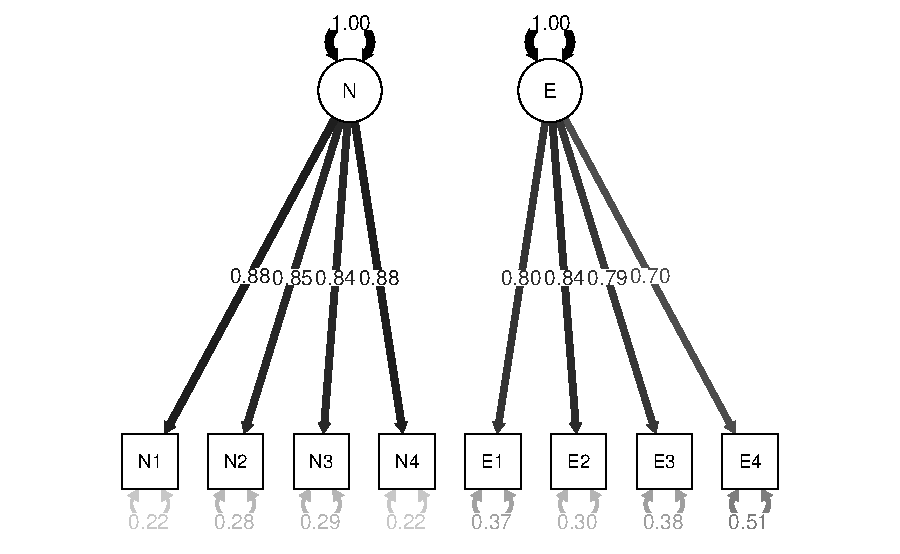
\includegraphics{cfa_book_files/figure-latex/unnamed-chunk-27-1} \end{center}

Come indicato nel diagramma, l'effetto diretto di \texttt{mom\_iq} su \texttt{kid\_score} è identico al corrispondente coefficiente parziale di regressione.

\hypertarget{errore-di-specificazione}{%
\subsection{Errore di specificazione}\label{errore-di-specificazione}}

Spiritosamente chiamato ``heartbreak of L.O.V.E.'' (Left-Out Variable Error; \citet{mauro1990understanding}), l'errore di specificazione è una caratteristica fondamentale dei modelli di regressione che deve sempre essere tenuta a mente quando interpretiamo i risultati di questa analisi statistica. L'errore di specificazione si verifica quando escludiamo dal modello di regressione una variabile che

\begin{itemize}
\tightlist
\item
  è associata con altre variabili nel modello,
\item
  ha un effetto diretto sulla \(y\).
\end{itemize}

Come conseguenza dell'errore di specificazione, la direzione e il segno dei coefficienti parziali di regressione risultano sistematicamente distorti.

Consideriamo un esempio con dati simulati nei quali immaginiamo che la prestazione sia positivamente associata alla motivazione e negativamente associata all'ansia. Immaginiamo inoltre che vi sia una correlazione positiva tra ansia a motivazione. Ci chiediamo cosa succede al coefficiente parziale della variabile ``motivazione'' se la variabile ``ansia'' viene esclusa dal modello di regressione.

\begin{Shaded}
\begin{Highlighting}[]
\FunctionTok{set.seed}\NormalTok{(}\DecValTok{123}\NormalTok{)}
\NormalTok{anxiety }\OtherTok{\textless{}{-}} \FunctionTok{rnorm}\NormalTok{(n, }\DecValTok{10}\NormalTok{, }\FloatTok{1.5}\NormalTok{)}
\NormalTok{motivation }\OtherTok{\textless{}{-}} \FloatTok{4.0} \SpecialCharTok{*}\NormalTok{ anxiety }\SpecialCharTok{+} \FunctionTok{rnorm}\NormalTok{(n, }\DecValTok{0}\NormalTok{, }\FloatTok{3.5}\NormalTok{)}
\FunctionTok{cor}\NormalTok{(anxiety, motivation)}
\CommentTok{\#\textgreater{} [1] 0.8435}
\end{Highlighting}
\end{Shaded}

\begin{Shaded}
\begin{Highlighting}[]
\NormalTok{performance }\OtherTok{\textless{}{-}} \FloatTok{0.5} \SpecialCharTok{*}\NormalTok{ motivation }\SpecialCharTok{{-}} \FloatTok{5.0} \SpecialCharTok{*}\NormalTok{ anxiety }\SpecialCharTok{+} \FunctionTok{rnorm}\NormalTok{(n, }\DecValTok{0}\NormalTok{, }\DecValTok{3}\NormalTok{)}
\end{Highlighting}
\end{Shaded}

\begin{Shaded}
\begin{Highlighting}[]
\NormalTok{sim\_dat2 }\OtherTok{\textless{}{-}} \FunctionTok{tibble}\NormalTok{(performance, motivation, anxiety)}
\NormalTok{fm1 }\OtherTok{\textless{}{-}} \FunctionTok{lm}\NormalTok{(performance }\SpecialCharTok{\textasciitilde{}}\NormalTok{ motivation }\SpecialCharTok{+}\NormalTok{ anxiety, sim\_dat2)}
\FunctionTok{coef}\NormalTok{(fm1)}
\CommentTok{\#\textgreater{} (Intercept)  motivation     anxiety }
\CommentTok{\#\textgreater{}      3.0686      0.5204     {-}5.3480}
\end{Highlighting}
\end{Shaded}

\begin{Shaded}
\begin{Highlighting}[]
\NormalTok{fm2 }\OtherTok{\textless{}{-}} \FunctionTok{lm}\NormalTok{(performance }\SpecialCharTok{\textasciitilde{}}\NormalTok{ motivation, sim\_dat2)}
\FunctionTok{summary}\NormalTok{(fm2)}
\CommentTok{\#\textgreater{} }
\CommentTok{\#\textgreater{} Call:}
\CommentTok{\#\textgreater{} lm(formula = performance \textasciitilde{} motivation, data = sim\_dat2)}
\CommentTok{\#\textgreater{} }
\CommentTok{\#\textgreater{} Residuals:}
\CommentTok{\#\textgreater{}     Min      1Q  Median      3Q     Max }
\CommentTok{\#\textgreater{} {-}12.110  {-}3.509   0.334   2.940  16.725 }
\CommentTok{\#\textgreater{} }
\CommentTok{\#\textgreater{} Coefficients:}
\CommentTok{\#\textgreater{}             Estimate Std. Error t value Pr(\textgreater{}|t|)    }
\CommentTok{\#\textgreater{} (Intercept) {-}11.7178     3.1592   {-}3.71  0.00034 ***}
\CommentTok{\#\textgreater{} motivation   {-}0.4610     0.0777   {-}5.93  4.5e{-}08 ***}
\CommentTok{\#\textgreater{} {-}{-}{-}}
\CommentTok{\#\textgreater{} Signif. codes:  }
\CommentTok{\#\textgreater{} 0 \textquotesingle{}***\textquotesingle{} 0.001 \textquotesingle{}**\textquotesingle{} 0.01 \textquotesingle{}*\textquotesingle{} 0.05 \textquotesingle{}.\textquotesingle{} 0.1 \textquotesingle{} \textquotesingle{} 1}
\CommentTok{\#\textgreater{} }
\CommentTok{\#\textgreater{} Residual standard error: 4.87 on 98 degrees of freedom}
\CommentTok{\#\textgreater{} Multiple R{-}squared:  0.264,  Adjusted R{-}squared:  0.257 }
\CommentTok{\#\textgreater{} F{-}statistic: 35.2 on 1 and 98 DF,  p{-}value: 4.51e{-}08}
\end{Highlighting}
\end{Shaded}

Il risultato prodotto dal modello di regressione è sbagliato: come conseguenza dell'errore di specificazione, il segno del coefficiente parziale di regressione della variabile ``motivazione'' è negativo, anche se nel vero modello di regressione tale coefficiente ha il segno opposto. Quindi, se noi interpretassimo il coefficiente parziale ottenuto in termini casuali, saremmo portati a concludere che la motivazione fa diminuire la prestazione anche se, in realtà (nel modello generatore dei dati), è vero l'opposto.

\hypertarget{soppressione}{%
\subsection{Soppressione}\label{soppressione}}

Le conseguenze dell'errore di specificazione sono chiamate ``soppressione'' (\emph{suppression}). In generale, si ha soppressione quando (1) il valore assoluto del peso beta di un predittore è maggiore di quello della sua correlazione bivariata con il criterio o (2) i due hanno segni opposti.

\begin{itemize}
\tightlist
\item
  L'esempio descritto sopra è un caso di \emph{soppressione negativa}, dove il predittore ha correlazioni bivariate positive con il criterio, ma si riceve un peso beta negativo nell'analisi di regressione multipla.
\item
  Un secondo tipo di soppressione è la \emph{soppressione classica}, in cui un predittore non è correlato al criterio ma riceve un peso beta diverso da zero se un altro predittore viene controllato.
\item
  C'è anche la \emph{soppressione reciproca} che può verificarsi quando due variabili sono correlate positivamente con il criterio ma negativamente tra loro.
\end{itemize}

\hypertarget{stepwise-regression}{%
\subsection{Stepwise regression}\label{stepwise-regression}}

Un'implicazione della soppressione è che i predittori non dovrebbero essere selezionati in base ai valori delle correlazioni bivariate con il criterio. Queste associazioni di ordine zero non controllano gli effetti degli altri predittori, quindi i loro valori possono essere fuorvianti rispetto ai coefficienti di regressione parziale per le stesse variabili. Per lo stesso motivo, il fatto che le correlazioni bivariate con il criterio siano statisticamente significative o meno è irrilevante per quanto riguarda la selezione dei predittori. Sebbene le procedure informatiche di regressione rendano facile tali processi di selezione dei predittori, i ricercatori dovrebbero evitare di usare tali metodi. Il rischio è che anche piccole, ma non rilevate, non-linearità o effetti indiretti tra i predittori possano seriamente distocere i coefficienti di regressione parziale. È meglio selezionare giudiziosamente il minor numero di predittori sulla base di ragioni teoriche o dei risultati di ricerche precedenti.

Una volta selezionati, ci sono due modi di base per inserire i predittori nell'equazione di regressione: uno consiste nell'inserire tutti i predittori contemporaneamente. L'altro è inserirli nel corso di una serie di passaggi, ovvero mediante usando una procedura sequenziale. L'ordine di ingresso può essere determinato in base a uno di due diversi standard: teorici (razionali) o empirici (statistici). Lo standard razionale corrisponde alla regressione gerarchica, in cui si comunica al computer un ordine fisso per inserire i predittori. Ad esempio, a volte le variabili demografiche vengono inserite nel primo passaggio, quindi nel secondo passaggio viene inserita una variabile psicologica di interesse. Questo ordine non solo controlla le variabili demografiche ma permette anche di valutare il potere predittivo della variabile psicologica, al di là di quello delle semplici variabili demografiche. Quest'ultimo può essere stimato come l'aumento della correlazione multipla al quadrato, o \(\Delta R^2\), da quella della fase 1 con solo predittori demografici a quella della fase 2 con tutti i predittori nell'equazione di regressione.

Un esempio di standard statistico è la regressione \emph{stepwise}, in cui il computer seleziona l'inserimento dei predittori in base esclusivamente alla significatività statistica; cioè, viene chiesto: quale predittore, se inserito nell'equazione, avrebbe il valore\_\(p\) più piccolo per il test del suo coefficiente di regressione parziale? Dopo la selezione, i predittori in una fase successiva possono essere rimossi dall'equazione di regressione in base ai loro valori-\(p\) (ad esempio, se \(p \geq\) .05). Il processo stepwise si interrompe quando, aggiungendo più predittori, \(\Delta R^2\) non migliora. Varianti della regressione stepwise includono \emph{forward inclusion}, in cui i predittori selezionati non vengono successivamente rimossi dal modello, e \emph{backward elimination}, che inizia con tutti i predittori nel modello per poi rimuoverne alcuni in passi successivi. I problemi relativi ai metodi stepwise sono così gravi da essere effettivamente banditi in alcuni giornali. Un problema è che fanno leva su risultati che si ottengono per caso, in dipendenza delle idiosincrasie del campione (quindi, non replicabili).

In secondo luogo, una volta che un insieme finale di predittori selezionati razionalmente è stato inserito nell'equazione di regressione, tali predittori non dovrebbero essere successivamente rimossi se i loro coefficienti di regressione non sono statisticamente significativi: il ricercatore non dovrebbe sentirsi in dovere di lasciar perdere ogni predittore che non risulta statisticamente significativo. In campioni piccoli, la potenza dei test di significatività è bassa e la rimozione di un predittore non significativo può alterare sostanzialmente la soluzione. Se c'è una buona ragione per includere un predittore, allora è meglio lasciarlo nel modello, fino a prova contraria.

\hypertarget{part-la-teoria-classica-dei-test}{%
\part{La teoria classica dei test}\label{part-la-teoria-classica-dei-test}}

\hypertarget{ch:teoria_classica}{%
\chapter{Fondamenti teorici}\label{ch:teoria_classica}}

\hypertarget{valutazione-psicometrica-come-ragionamento-inferenziale}{%
\section{Valutazione psicometrica come ragionamento inferenziale}\label{valutazione-psicometrica-come-ragionamento-inferenziale}}

In apparenza, i test psicometrici sono solo dei test. Somministriamo un test, otteniamo un punteggio ed è naturale pensare che sia tutto lì. Nonostante le apparenze, la valutazione psicologica e neuropsicologica non consiste soltanto nell'assegnare di punteggi: si tratta di ragionare su ciò che osserviamo di quello che le persone dicono, fanno o producono, in maniera tale da giungere a delle concezioni più ampie di tali persone a proposito di aspetti che non abbiamo -- e spesso non possiamo -- osservare. Più specificamente, possiamo considerare la valutazione psicologica e neuropsicologica come un esempio di ragionamento che fa uso di modelli probabilistici per giungere a delle spiegazioni, previsioni o conclusioni.

I dati osservati diventano un'evidenza quando sono ritenuti rilevanti per l'inferenza desiderata attraverso l'instaurazione di relazioni tra i dati e l'obiettivo dell'inferenza. Spesso utilizziamo dati provenienti da più fonti. Queste possono essere di tipo simile (ad esempio, item di test aventi lo stesso formato) o di tipo molto diverso (ad esempio, il curriculum di un richiedente oltre al colloquio, la storia medica della famiglia di un paziente, \(\dots\)). Le evidenze possono essere contraddittorie (ad esempio, uno studente riesce a svolgere un compito difficile ma fallisce in un uno facile) e quasi sempre non sono del tutto conclusive.

Queste caratteristiche hanno due implicazioni. In primo luogo, è difficile capire cosa le evidenze implicano. I processi inferenziali sono sempre complessi. In secondo luogo, a causa della natura non conclusiva delle evidenze disponibili, non siamo mai del tutto certi delle nostre inferenze. Per affrontare tale incertezza, la teoria psicometria ci fornisce gli strumenti che ci possono aiutare nel processo inferenziale, dai dati disponibili alle decisioni che prendiamo.

Un secolo fa, la relazione tra prestazioni osservate, da un lato, e l'abilità inosservabile del rispondente, dall'altro, iniziò a essere formalizzata nei termini dell'\emph{errore di misurazione}. \citet{gulliksen1961measurement} ha descritto ``il problema centrale della teoria dei test'' come ``la relazione tra l'abilità dell'individuo e il suo punteggio osservato sul test'' (p.~101). Tale caratterizzazione è valida ancora oggi, con una definizione opportunamente ampia di ``abilità'' e di ``punteggio sul test'' che sia in grado di comprendere le diverse forme di assessment psicologico e neuropsicologico. Comprendere e essere in grado di rappresentare la relazione tra le prestazioni osservate e la capacità soggiacente è dunque fondamentale per le forme di ragionamento che vengono impiegate nella valutazione psicologica e neuropsicologica.

Come risultato dell'errore di misurazione, i ragionamenti che compiamo nella valutazione psicologica e neuropsicologica costituiscono un esempio di ragionamento in condizioni di incertezza. A causa della natura imperfetta della misurazione e dell'incompletezza dell'informazione disponibile, le nostre inferenze sono incerte e possono essere sempre invalidate o riviste. Ragionare da ciò che è parziale (ciò che vediamo uno paziente dire, fare o produrre) a ciò che è generale (la ``vera'' abilità del paziente) è necessariamente incerto, e le nostre inferenze o conclusioni sono sempre prone ad errori.

Quali strumenti devono essere impiegati per affrontare la nostra incertezza sulla relazione che intercorre tra prestazioni osservate e abilità soggiacenti? Secondo Lewis, molti dei progressi nella teoria psicometrica sono resi possibili ``trattando lo studio della relazione tra le risposte agli item di un test e il tratto ipotizzato di un individuo come problema di inferenza statistica'' \citep{lewis1986test}. Una connessione diretta tra errore di misura e approccio probabilistico è stata anche proposta da Samejima: ``There may be an enormous number of factors eliciting a student's specific overt reactions to a stimulus, and, therefore, it is suitable, even necessary, to handle the situation in terms of the probabilistic relationship between the two'' \citep{samejima1983constant}.

Questo punto di vista è diventato quello dominante nella psicometria moderna e sottolinea l'utilità di utilizzare il linguaggio e gli strumenti della teoria della probabilità per comunicare il carattere parziale dei dati di cui dispone lo psicologo e l'incertezza delle inferenze che ne derivano.

I reattivi psicologici possono essere costruiti e la validati mediante vari approcci probabilistici: la Teoria Classica dei test (\emph{classical test theory}, in breve CTT) e la teoria di risposta all'item (\emph{item response theory}, in breve IRT) sono quelli più noti. Recentemente, il problema della valutazione psicologica è stato anche formulato in un'ottica bayesiana. In questo insegnamento esamineremo gli approcci della CTT e dell'IRT, ma non quello bayesiano.

\hypertarget{la-teoria-classica}{%
\section{La Teoria Classica}\label{la-teoria-classica}}

La CTT nasce alla fine dell'Ottocento (Alfred Binet e altri, 1894) allo scopo di studiare l'attendibilità e la validità dei risultati dei questionari utilizzati per valutare le caratteristiche psico-sociali, non direttamente osservabili, delle persone esaminate. L'impiego su vasta scala e lo sviluppo della CTT ha inizio negli anni Trenta, anche se il modello formale su cui tale teoria si basa viene proposta da Spearman all'inizio del Novecento \citep{ch1904general}. La tecnica dell'analisi fattoriale esplorativa (\emph{Exploratory Factor Analysis}, EFA), verrà poi affinata da \citet{thurstone1947multiple} alla fine della seconda guerra mondiale. Tra la fine degli anni '60 e gli inizi degli anni '70, \citet{joreskog1969general} sviluppa l'analisi fattoriale confermativa (\emph{Confirmatory Factor Analysis}, CFA). Negli anni '70, l'analisi fattoriale viene integrata con la path analysis nel lavoro di \citet{joreskog1978structural} che dà origine ai modelli di equazioni strutturali (\emph{Structural Equation Modeling}, SEM).

Iniziamo qui ad esaminare queste tecniche psicometriche prendendo in esame, per prima, la teoria classica dei test. Seguiremo la trattazione proposta da \citet{lord1968statistical}.

L'equazione fondamentale alla quale si riconduce la teoria classica dei test è quella che ipotizza una relazione lineare e additiva tra il punteggio osservato di un test (\(X\)), la misura della variabile latente (\(T\)) e la componente casuale dell'errore (\(E\)). Un punto cruciale nella CTT è l'entità della varianza dell'errore. Minore è la varianza dell'errore, più accuratamente il punteggio reale viene riflesso dai nostri punteggi osservati. In un mondo perfetto, tutti i valori di errore sarebbero uguali a 0. Cioè, ogni partecipante otterrebbe il punteggio esatto. Questo però non è possibile. Pertanto, abbiamo una certa varianza negli errori. La corrispondente deviazione standard di tali errori ha il un nome: si chiama \emph{errore standard di misurazione}, indicato da \(\sigma_E\). Uno dei principali obiettivi della CTT è quello di ottenere una stima di \(\sigma_E\).

\hypertarget{le-due-componenti-del-punteggio-osservato}{%
\section{Le due componenti del punteggio osservato}\label{le-due-componenti-del-punteggio-osservato}}

CTT si occupa delle relazioni tra \(X\), \(T\) ed \(E\). La CTT si basa su un modello relativamente semplice in cui il punteggio osservato, il punteggio vero (cioè l'abilità inosservabile del rispondente) e l'errore aleatoria di misurazione sono legati da una relazione lineare. Indicati con \(T_{\nu j}\) (\emph{true score}) l'abilità latente da misurare dell'individuo \(\nu\) nella prova \(j\), con \(X_{\nu j}\) la variabile osservata (\emph{observed score}) per l'individuo \(\nu\) nella prova \(j\) e con \(E_{\nu j}\) l'errore aleatorio di misurazione, il modello si rappresenta con

\[
X_{\nu j} = T_{\nu} + E_{\nu j}. 
\label{eq:observed-true-plus-error}
\]

Dunque, in base alla \eqref{eq:observed-true-plus-error} il punteggio osservato \(X_{\nu j}\) differisce da quello vero \(T_{\nu j}\) a causa di una componente di errore aleatoria \(E_{\nu j}\). Uno degli obiettivi centrali della CTT è quello di quantificare l'entità di tale errore. Vedremo come questa quantificazione verrà fornita nei termini dell'attendibilità del test. L'attendibilità (o affidabilità) rappresenta l'accuratezza con cui un test può misurare il punteggio vero (Coaley, 2014):

\begin{itemize}
\tightlist
\item
  Se l'attendibilità è grande, \(\sigma_E\) è piccolo: \(X\) ha un piccolo errore di misurazione e sarà vicino a \(T\).
\item
  Se l'attendibilità è piccola, \(\sigma_E\) è grande: \(X\) presenta un grande errore di misurazione e si discosterà molto da \(T\).
\end{itemize}

\hypertarget{il-punteggio-vero}{%
\subsection{Il punteggio vero}\label{il-punteggio-vero}}

La @ref(eq:observed-true\_plus-error) ci dice che il punteggio osservato è dato dalla somma di due componenti: una componente sistematica (il punteggio vero) e una componente aleatoria (l'errore di misurazione). Ma che cos'è il punteggio vero? La CTT considera un reattivo psicologico come una selezione aleatoria di item da un universo/popolazione di item attinenti al costrutto da misurare \citep{nunnally1994psychometric, kline2013handbook}. Se il reattivo psicologico viene concepito in questo modo, il punteggio vero diventa il punteggio che un rispondente otterrebbe se fosse misurato su tutto l'universo degli item proprio del costrutto in esame. L'errore di misurazione riflette dunque il grado in cui gli item che costituiscono il test non riescono a rappresentare l'intero universo degli item attinenti al costrutto.

In maniera equivalente, il punteggio vero può essere concepito come il punteggio non ``distorto'' da componenti estranee al costrutto, ovvero da effetti di apprendimento, fatica, memoria, motivazione, eccetera. Essendo concepita come del tutto aleatoria (ovvero, priva di qualunque natura sistematica), la componente aleatoria non introduce dei bias nella tendenza centrale della misurazione.

Il punteggio vero è concepito come un punteggio inosservabile che corrisponde al valore atteso di infinite realizzazioni del punteggio ottenuto:

\[
T = \E(X) \equiv \mu_X \equiv \mu_{T}.
\]

In altri termini, secondo la definizione di Lord e Novick (1968), e facendo riferimento a alla seconda definizione presentata sopra, il punteggio vero è concepito come la media dei punteggi che un soggetto otterrebbe se il test venisse somministrato ripetutamente nelle stesse condizioni, in assenza di effetti di apprendimento e/o fatica.

\hypertarget{somministrazioni-ripetute}{%
\subsection{Somministrazioni ripetute}\label{somministrazioni-ripetute}}

Nella formulazione del modello della CTT si possono distinguere due tipi di esperimenti aleatori: uno che considera l'unità di osservazione (l'individuo) come campionaria, l'altro che considera il punteggio, per un determinato individuo, come campionario. Un importante risultato è dato dall'unione dei due esperimenti, ovvero dalla dimostrazione che i risultati della CTT, la quale è stata sviluppata ipotizzando ipotetiche somministrazioni ripetute del test allo stesso individuo sotto le medesime condizioni, si generalizzano al caso di una singola somministrazione del test ad un campione di individui \citep{allen2001introduction}. In base a questo risultato, se consideriamo la somministrazione del test ad una popolazione di individui, allora diventa più facile dare un contenuto empirico alle quantità della CTT:

\begin{itemize}
\tightlist
\item
  \(\sigma^2_X\) è la varianza del punteggio osservato nella popolazione,
\item
  \(\sigma^2_T\) è la varianza dei punteggio vero nella popolazione,
\item
  \(\sigma^2_E\) è la varianza della componente d'errore nella popolazione.
\end{itemize}

\hypertarget{le-assunzioni-sul-punteggio-ottenuto}{%
\subsection{Le assunzioni sul punteggio ottenuto}\label{le-assunzioni-sul-punteggio-ottenuto}}

La CTT \emph{assume} che la media del punteggio osservato \(X\) sia uguale alla media del punteggio vero,

\[
\mu_X \equiv \mu_{T},
\label{eq:assunzione-media-x-media-t}
\]

in altri termini, assume che il punteggio osservato fornisca una stima statisticamente corretta dell'abilità latente (punteggio vero). In pratica, il punteggio osservato non sarà mai uguale all'abilità latente, ma corrisponde solo ad uno dei possibili punteggi che il soggetto può ottenere, subordinatamente alla sua abilità latente. L'errore della misura è la differenza tra il punteggio osservato e il punteggio vero: \(E \equiv X - T.\)

In base all'assunzione secondo cui il valore atteso dei punteggi è uguale alla media del valore vero, segue che

\[
\E(E) = \E(X - T) = \E(X) - \E(T) = \mu_{T} - \mu_{T} = 0,
\]

ovvero, il valore atteso degli errori è uguale a zero.

\hypertarget{lerrore-standard-della-misurazione-sigma_e}{%
\section{\texorpdfstring{L'errore standard della misurazione \(\sigma_E\)}{L'errore standard della misurazione \textbackslash sigma\_E}}\label{lerrore-standard-della-misurazione-sigma_e}}

La radice quadrata di \(\sigma^2_E\), ovvero la deviazione standard degli errori, è la quantità fondamentale della CTT ed è chiamata \emph{errore standard della misurazione}. La stima dell'errore standard della misurazione costituisce uno degli obiettivi più importanti della CTT. Ricordiamo che la deviazione standard è simile (non identica) alla media del valore assoluto degli scarti dei valori di una distribuzione dalla media. Possiamo dunque utilizzare questa proprietà per descrivere il modo in cui la CTT interpreta \(\sigma_E\).

L'\emph{errore standard della misurazione} \(\sigma_E\) ci dice qual è, approssimativamente, la variazione attesa del punteggio osservato, se il test venisse somministrato un'altra volta al rispondente nelle stesse condizioni.

\hypertarget{assiomi-della-teoria-classica}{%
\section{Assiomi della Teoria Classica}\label{assiomi-della-teoria-classica}}

La CTT \emph{assume} che gli errori siano delle variabili aleatorie incorrelate tra loro

\[
\rho(E_i, E_k \mid T) = 0, \qquad\text{con}\; i \neq k,
\]

e incorrelate con il punteggio vero,

\[
\rho(E, T) = 0,
\]

le quali seguono una distribuzione gaussiana con media zero e deviazione standard pari a \(\sigma_E\):

\[
E \sim \mathcal{N}(0, \sigma_E).
\]

La quantità \(\sigma_E\) è detta errore standard della misurazione.

Sulla base di tali assunzioni la CTT deriva la formula dell'attendibilità di un test. Si noti che le assunzioni della CTT hanno una corrispondenza puntuale con le assunzioni su cui si basa il modello di regressione lineare.

\hypertarget{lattendibilituxe0-del-test}{%
\section{L'attendibilità del test}\label{lattendibilituxe0-del-test}}

Il concetto di attendibilità è strettamente legato alla riproducibilità della misurazione: si riferisce al grado di stabilità, di coerenza interna e di precisione di una procedura di misurazione. Affinché una misurazione psicologica sia utile, deve produrre lo stesso risultato se viene applicata ripetutamente un determinato rispondente. Altri termini che vengono usati sono: affidabilità, costanza e credibilità.

Vedremo nel seguito come il coefficiente di attendibilità fornisce una stima della quota della varianza del punteggio osservato che può essere attribuita all'abilità latente (``punteggio vero'', cioè privo di errore di misurazione). In generale, un coefficiente di attendibilità maggiore di 0.80 viene ritenuto soddisfacente perché indica che l'80\% o più della varianza dei punteggi ottenuti è causata da ciò che il test intende misurare, anziché dall'errore di misurazione.

Per definire l'attendibilità, la CTT si serve di due quantità:

\begin{itemize}
\tightlist
\item
  la varianza del punteggio osservato,
\item
  la correlazione tra punteggio osservato e punteggio vero.
\end{itemize}

Vediamo come queste quantità possano essere ottenute sulla base delle assunzioni del modello statistico che sta alla base della CTT.

\hypertarget{la-varianza-del-punteggio-osservato}{%
\subsection{La varianza del punteggio osservato}\label{la-varianza-del-punteggio-osservato}}

La varianza del punteggio osservato \(X\) è uguale alla somma della varianza del punteggio vero e della varianza dell'errore di misurazione.

\begin{proof}
La varianza del punteggio osservato è uguale a

\[
\sigma^2_X =  \V(T+E) =  \sigma_T^2 + \sigma_E^2 + 2 \sigma_{TE}.
\label{eq:3-2-4}
\]

Dato che \(\sigma_{TE}=\rho_{TE}\sigma_T \sigma_E=0\), in quanto \(\rho_{TE}=0\), ne segue che

\[
\sigma^2_X =   \sigma_T^2 + \sigma_E^2.
\label{eq:var-sum}
\]
\end{proof}

\hypertarget{la-covarianza-tra-punteggio-osservato-e-punteggio-vero}{%
\subsection{La covarianza tra punteggio osservato e punteggio vero}\label{la-covarianza-tra-punteggio-osservato-e-punteggio-vero}}

La covarianza tra punteggio osservato \(X\) e punteggio vero \(T\) è uguale alla varianza del punteggio vero.

\begin{proof}
\begin{equation}
\begin{aligned}
\sigma_{X T} &= \E(XT) - \E(X)\E(T)\notag\\
&=  \E[(T+E)T] - \E(T+E)\E(T)\notag\\
&=  \E(T^2) + \underbrace{\E(ET)}_{=0} - [\E(T)]^2 -  \underbrace{\E(E)}_{=0} \E(T)\notag\\
&=\E(T^2) - [\E(T)]^2\notag \\
&= \sigma_T^2.
\end{aligned}
\end{equation}
\end{proof}

Da ciò segue che la correlazione tra punteggio osservato \(X\) e punteggio vero \(T\) è uguale al rapporto tra la deviazione standard del punteggio vero e la deviazione standard del punteggio osservato:

\begin{equation}
\begin{aligned}
\rho_{XT} &= \frac{\sigma_{XT}}{\sigma_X \sigma_T} = \frac{\sigma^2_{T}}{\sigma_X \sigma_T} = \frac{\sigma_{T}}{\sigma_X}.
\label{eq:sd-ratio}
\end{aligned}
\end{equation}

\hypertarget{definizione-e-significato-dellattendibilituxe0}{%
\subsection{Definizione e significato dell'attendibilità}\label{definizione-e-significato-dellattendibilituxe0}}

La CTT definisce attendibilità di un test (o di un item) come il quadrato della correlazione tra punteggio osservato \(X\) e punteggio vero \(T\), ovvero come il rapporto tra la varianza del punteggio vero e la varianza del punteggio osservato:

\[
\rho_{XT}^2 = \frac{\sigma_{T}^2}{\sigma_X^2}.
\label{eq:reliability-1}
\]

Questa è la quantità fondamentale della CTT e misura il grado di variazione del punteggio vero rispetto alla variazione del punteggio osservato{[}\^{}2{]}.

Dato che \(\sigma^2_X = \sigma_T^2 + \sigma_E^2\), in base alla \eqref{eq:reliability-1} possiamo scrivere

\begin{equation}
\begin{aligned}
\rho_{XT}^2 &= \frac{\sigma_{T}^2}{\sigma_X^2} =\frac{\sigma_{X}^2 - \sigma^2_E}{\sigma_X^2}
 = 1-\frac{\sigma_{E}^2}{\sigma_X^2}.
 \label{eq:3-2-6}
\end{aligned}
\end{equation}

Questo significa che il coefficiente di attendibilità assume valore \(1\) se la varianza degli errori \(\sigma_{E}^2\) è nulla e assume valore \(0\) se la varianza degli errori è uguale alla varianza del punteggio osservato. Ciò significa che il coefficiente di attendibilità è un numero contenuto nell'intervallo compreso tra \(0\) e \(1\).

\hypertarget{attendibilituxe0-e-modello-di-regressione-lineare}{%
\section{Attendibilità e modello di regressione lineare}\label{attendibilituxe0-e-modello-di-regressione-lineare}}

Il modello di regressione lineare sta alla base della CTT. Infatti si può dire che tutte le proprietà della CTT che abbiamo discusso in precedenza non sono altro che le caratteristiche di un modello di regressione lineare nel quale

\begin{itemize}
\tightlist
\item
  la variabile dipendente è costituita dai punteggi osservati \(X\), e
\item
  la variabile indipendente corrisponde ai punteggi veri \(T\).
\end{itemize}

Se rappresentiamo la CTT in questo modo, il coefficiente di attendibilità \(\rho_{XT}^2 = \frac{\sigma_{T}^2}{\sigma_X^2}\) non diventa altro che la quota di varianza del punteggio osservato \(X\) che viene spiegata dal punteggio vero \(T\) in base ad un modello lineare con pendenza unitaria e intercetta nulla. Nei termini di una tale rappresentazione, il coefficiente di attendibilità misura la forza della relazione lineare tra \(X\) e \(T\) e corrisponde al coefficiente di determinazione del seguente modello di regressione:

\[
X = 0 + 1 \cdot T + E.
\]

\hypertarget{simulazione}{%
\subsection{Simulazione}\label{simulazione}}

Per dare un contenuto concreto alle affermazioni precedenti, consideriamo la seguente simulazione svolta in . In tale simulazione il punteggio vero \(T\) e l'errore \(E\) verranno creati in modo tale da soddisfare i due vincoli della CTT: \(T\) e \(E\) saranno delle variabili gaussiane e tra loro incorrelate. Nella simulazione generiamo 100 coppie di valori \(X\) e \(T\) con i seguenti parametri: \(T \sim \mathcal{N}(\mu_T = 12, \sigma^2_T = 6)\), \(E \sim \mathcal{N}(\mu_E = 0, \sigma^2_T = 3)\). A tale fine usiamo le seguenti istruzioni:

\begin{Shaded}
\begin{Highlighting}[]
\FunctionTok{set.seed}\NormalTok{(}\DecValTok{123}\NormalTok{)}
\FunctionTok{library}\NormalTok{(}\StringTok{"MASS"}\NormalTok{)}
\NormalTok{n }\OtherTok{\textless{}{-}} \DecValTok{100}
\NormalTok{Sigma }\OtherTok{\textless{}{-}} \FunctionTok{matrix}\NormalTok{(}\FunctionTok{c}\NormalTok{(}\DecValTok{6}\NormalTok{, }\DecValTok{0}\NormalTok{, }\DecValTok{0}\NormalTok{, }\DecValTok{3}\NormalTok{), }\AttributeTok{byrow =} \ConstantTok{TRUE}\NormalTok{, }\AttributeTok{ncol =} \DecValTok{2}\NormalTok{)}
\NormalTok{Sigma}
\CommentTok{\#\textgreater{}      [,1] [,2]}
\CommentTok{\#\textgreater{} [1,]    6    0}
\CommentTok{\#\textgreater{} [2,]    0    3}
\end{Highlighting}
\end{Shaded}

\begin{Shaded}
\begin{Highlighting}[]
\NormalTok{mu }\OtherTok{\textless{}{-}} \FunctionTok{c}\NormalTok{(}\DecValTok{12}\NormalTok{, }\DecValTok{0}\NormalTok{)}
\NormalTok{mu}
\CommentTok{\#\textgreater{} [1] 12  0}
\end{Highlighting}
\end{Shaded}

\begin{Shaded}
\begin{Highlighting}[]
\NormalTok{Y }\OtherTok{\textless{}{-}} \FunctionTok{mvrnorm}\NormalTok{(n, mu, Sigma, }\AttributeTok{empirical =} \ConstantTok{TRUE}\NormalTok{)}
\NormalTok{T }\OtherTok{\textless{}{-}}\NormalTok{ Y[, }\DecValTok{1}\NormalTok{]}
\NormalTok{E }\OtherTok{\textless{}{-}}\NormalTok{ Y[, }\DecValTok{2}\NormalTok{]}
\end{Highlighting}
\end{Shaded}

Le istruzioni precedenti creano un insieme di valori tali per cui le medie e la matrice di varianze-covarianze assumono esattamente i valori indicati. Possiamo dunque immaginare tale insieme di dati come la nostra ``popolazione''.

Secondo la CTT, il punteggio osservato è \(X = T + E\). Simuliamo dunque il punteggio osservato \(X\) nel modo seguente:

\begin{Shaded}
\begin{Highlighting}[]
\NormalTok{X }\OtherTok{\textless{}{-}}\NormalTok{ T }\SpecialCharTok{+}\NormalTok{ E}
\end{Highlighting}
\end{Shaded}

Le prime 6 osservazioni così ottenute sono:

\begin{Shaded}
\begin{Highlighting}[]
\FunctionTok{head}\NormalTok{(}\FunctionTok{cbind}\NormalTok{(T, E, X))}
\CommentTok{\#\textgreater{}           T       E      X}
\CommentTok{\#\textgreater{} [1,] 11.148 {-}1.5708  9.577}
\CommentTok{\#\textgreater{} [2,] 13.138 {-}0.3335 12.804}
\CommentTok{\#\textgreater{} [3,] 10.391  2.5457 12.937}
\CommentTok{\#\textgreater{} [4,] 11.452 {-}0.1955 11.257}
\CommentTok{\#\textgreater{} [5,]  9.978 {-}0.4920  9.486}
\CommentTok{\#\textgreater{} [6,] 10.730  2.9609 13.691}
\end{Highlighting}
\end{Shaded}

Un diagramma di dispersione è fornito nella figura seguente:

\begin{Shaded}
\begin{Highlighting}[]
\FunctionTok{tibble}\NormalTok{(X, T) }\SpecialCharTok{\%\textgreater{}\%}
  \FunctionTok{ggplot}\NormalTok{(}\FunctionTok{aes}\NormalTok{(X, T)) }\SpecialCharTok{+}
  \FunctionTok{geom\_point}\NormalTok{()}
\end{Highlighting}
\end{Shaded}

\begin{figure}

{\centering 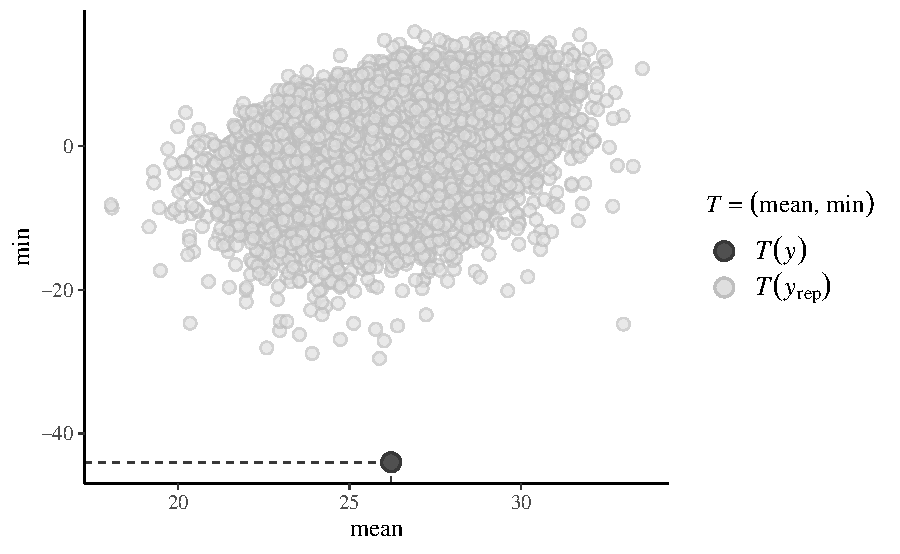
\includegraphics{cfa_book_files/figure-latex/unnamed-chunk-38-1} 

}

\caption{Simulazione della relazione tra punteggio osservato e punteggio vero per 100 individui in base alle assunzioni della CTT.}\label{fig:unnamed-chunk-38}
\end{figure}

Secondo la CTT, il valore atteso di \(T\) è uguale al valore atteso di \(X\). Verifichiamo questa assunzione della CTT nei nostri dati:

\begin{Shaded}
\begin{Highlighting}[]
\FunctionTok{mean}\NormalTok{(T)}
\CommentTok{\#\textgreater{} [1] 12}
\FunctionTok{mean}\NormalTok{(X)}
\CommentTok{\#\textgreater{} [1] 12}
\end{Highlighting}
\end{Shaded}

L'errore deve avere media zero, varianza \(\sigma_E^2\) e deve essere incorrelato con \(T\):

\begin{Shaded}
\begin{Highlighting}[]
\FunctionTok{mean}\NormalTok{(E)}
\CommentTok{\#\textgreater{} [1] 4.061e{-}18}
\FunctionTok{var}\NormalTok{(E)}
\CommentTok{\#\textgreater{} [1] 3}
\FunctionTok{cor}\NormalTok{(T, E)}
\CommentTok{\#\textgreater{} [1] {-}1.947e{-}16}
\end{Highlighting}
\end{Shaded}

Ricordiamo che la radice quadrata della varianza degli errori è chiamata errore standard della misurazione, \(\sigma_E\). La quantità \(\sqrt{\sigma_E^2}\) fornisce una misura della dispersione del punteggio osservato attorno al valore vero, nella condizione ipotetica di effettuare ripetute somministrazioni del test.

\begin{Shaded}
\begin{Highlighting}[]
\FunctionTok{sqrt}\NormalTok{(}\DecValTok{3}\NormalTok{)}
\CommentTok{\#\textgreater{} [1] 1.732}
\end{Highlighting}
\end{Shaded}

Dato che \(T\) e \(E\) sono incorrelati, ne segue che la varianza del punteggio osservato \(X\) è uguale alla somma della varianza del punteggio vero \(T\) e della varianza degli errori \(E\):

\begin{Shaded}
\begin{Highlighting}[]
\FunctionTok{var}\NormalTok{(X)}
\CommentTok{\#\textgreater{} [1] 9}
\FunctionTok{var}\NormalTok{(T) }\SpecialCharTok{+} \FunctionTok{var}\NormalTok{(E)}
\CommentTok{\#\textgreater{} [1] 9}
\end{Highlighting}
\end{Shaded}

La varianza del punteggio vero \(T\) è uguale alla covarianza tra il punteggio vero \(T\) e il punteggio osservato \(X\):

\begin{Shaded}
\begin{Highlighting}[]
\FunctionTok{cov}\NormalTok{(T, X)}
\CommentTok{\#\textgreater{} [1] 6}
\FunctionTok{var}\NormalTok{(T)}
\CommentTok{\#\textgreater{} [1] 6}
\end{Highlighting}
\end{Shaded}

La correlazione tra il punteggio osservato e il punteggio vero è uguale al rapporto tra la deviazione standard del punteggio vero e la deviazione standard del punteggio osservato:

\begin{Shaded}
\begin{Highlighting}[]
\FunctionTok{cor}\NormalTok{(X, T)}
\CommentTok{\#\textgreater{} [1] 0.8165}
\FunctionTok{sd}\NormalTok{(T) }\SpecialCharTok{/} \FunctionTok{sd}\NormalTok{(X)}
\CommentTok{\#\textgreater{} [1] 0.8165}
\end{Highlighting}
\end{Shaded}

Focalizziamoci ora sull'attendibiiltà. Per la CTT, l'attendibilità è uguale al quadrato del coefficiente di correlazione tra il punteggio vero \(T\) e il punteggio osservato \(X\):

\begin{Shaded}
\begin{Highlighting}[]
\FunctionTok{cor}\NormalTok{(X, T)}\SpecialCharTok{\^{}}\DecValTok{2}
\CommentTok{\#\textgreater{} [1] 0.6667}
\end{Highlighting}
\end{Shaded}

La motivazione di questa simulazione è quella di mettere in relazione il coefficiente di attendibilità, calcolato con le formule della CTT, con il modello di regressione lineare. Analizziamo dunque i dati della simulazione mediante il seguente modello di regressione lineare:

\[
X = a + b T + E
\]

\begin{Shaded}
\begin{Highlighting}[]
\NormalTok{fm }\OtherTok{\textless{}{-}} \FunctionTok{lm}\NormalTok{(X }\SpecialCharTok{\textasciitilde{}}\NormalTok{ T)}
\FunctionTok{summary}\NormalTok{(fm)}
\CommentTok{\#\textgreater{} }
\CommentTok{\#\textgreater{} Call:}
\CommentTok{\#\textgreater{} lm(formula = X \textasciitilde{} T)}
\CommentTok{\#\textgreater{} }
\CommentTok{\#\textgreater{} Residuals:}
\CommentTok{\#\textgreater{}    Min     1Q Median     3Q    Max }
\CommentTok{\#\textgreater{} {-}4.197 {-}1.101  0.052  1.155  4.239 }
\CommentTok{\#\textgreater{} }
\CommentTok{\#\textgreater{} Coefficients:}
\CommentTok{\#\textgreater{}             Estimate Std. Error t value Pr(\textgreater{}|t|)    }
\CommentTok{\#\textgreater{} (Intercept) 8.53e{-}15   8.75e{-}01       0        1    }
\CommentTok{\#\textgreater{} T           1.00e+00   7.14e{-}02      14   \textless{}2e{-}16 ***}
\CommentTok{\#\textgreater{} {-}{-}{-}}
\CommentTok{\#\textgreater{} Signif. codes:  }
\CommentTok{\#\textgreater{} 0 \textquotesingle{}***\textquotesingle{} 0.001 \textquotesingle{}**\textquotesingle{} 0.01 \textquotesingle{}*\textquotesingle{} 0.05 \textquotesingle{}.\textquotesingle{} 0.1 \textquotesingle{} \textquotesingle{} 1}
\CommentTok{\#\textgreater{} }
\CommentTok{\#\textgreater{} Residual standard error: 1.74 on 98 degrees of freedom}
\CommentTok{\#\textgreater{} Multiple R{-}squared:  0.667,  Adjusted R{-}squared:  0.663 }
\CommentTok{\#\textgreater{} F{-}statistic:  196 on 1 and 98 DF,  p{-}value: \textless{}2e{-}16}
\end{Highlighting}
\end{Shaded}

Si noti che la retta di regressione ha intercetta 0 e pendenza 1. Questo è coerente con l'assunzione \(\E(X) = \E(T)\). Ma il risultato più importante di questa simulazione è il seguente: il coefficiente di determinazione (\(R^2\) = 0.67) del modello di regressione \(X = 0 + 1 \times T + E\) è identico al coefficiente di attendibilità che abbiamo calcolato con la formula \(\rho_{XT}^2 = \frac{\sigma_{T}^2}{\sigma_X^2}\):

\begin{Shaded}
\begin{Highlighting}[]
\FunctionTok{var}\NormalTok{(T) }\SpecialCharTok{/} \FunctionTok{var}\NormalTok{(X)}
\CommentTok{\#\textgreater{} [1] 0.6667}
\end{Highlighting}
\end{Shaded}

Ciò ci consente di attribuire al coefficiente di attendibilità la seguente interpretazione: l'attendibilità di un test non è altro che la quota di varianza del punteggio osservato \(X\) che viene spiegata dalla regressione di \(X\) sul punteggio vero \(T\) in un modello di regressione dove \(\alpha\) = 0 e \(\beta\) = 1.

Che cosa si può concludere dai risultati di questa simulazione? Possiamo dire che, in base alla CTT,

\begin{itemize}
\tightlist
\item
  c'è una relazione lineare tra il punteggio osservato \(X\) e il punteggio vero \(T\); tale relazione lineare ha pendenza unitaria e intercetta zero.
\item
  La CTT fa proprie le assunzioni del modello di regressione lineare: incorrelazione tra variabile esplicativa \(T\) ed errore \(E\), e indipendenza e gaussianità degli errori.
\item
  Come conseguenza di tali assunzioni, il coefficiente di attendibilità non è altro che la quota di varianza del punteggio osservato \(X\) che viene spiegata dal punteggio vero tramite una regressione lineare, ovvero non è altro che il coefficiente di determinazione del modello di regressione \(X = \alpha + \beta T + E,\) dove \(\alpha\) = 0 e \(\beta\) = 1.
\end{itemize}

Vedremo in seguito come sia possibile formulare la CTT nei termini del modello statistico dell'analisi fattoriale. Nel linguaggio dell'analisi fattoriale, la varianza dell'errore \(\sigma^2_E\) viene chiamata \emph{specificità} (\emph{uniqueness}).

\hypertarget{misurazioni-parallele-e-affidabilituxe0}{%
\section{Misurazioni parallele e affidabilità}\label{misurazioni-parallele-e-affidabilituxe0}}

L'equazione \(\rho_{XT}^2 = \frac{\sigma_{T}^2}{\sigma_X^2}\) definisce il coefficiente di attendibilità ma non fornisce gli strumenti per calcolarlo, dato che la varianza del punteggio vero \(\sigma_{T}^2\) è una quantità incognita. Il metodo utilizzato dalla CTT per ottenere una stima (empirica) dell'attendibilità è quello delle forme parallele del test. Se è possibile elaborare versioni alternative dello stesso test che risultino equivalenti tra loro in termini di contenuto, modalità di risposta e caratteristiche statistiche, allora diventa anche possibile stimare il coefficiente di attendibilità.

Secondo la CTT, due test \(X=T+E\) e \(X^\prime=T^\prime+E^\prime\) si dicono misurazioni parallele della stessa abilità latente se il punteggio vero \(T\) è uguale al punteggio vero \(T^\prime\) e se la varianza degli errori \(\V(E)\) è uguale alla varianza degli errori \(\V(E^\prime)\).

Se il punteggio vero è uguale al valore atteso del punteggio osservato, \(T = \E(X)\), allora devono essere uguali anche le medie dei punteggi osservati delle due forme parallele del test, \(\E(X) = \E(X^\prime)\).

\begin{proof}
Consideriamo l'eguaglianza dei valori attesi dei punteggi osservati in due forme parallele del test: \(\E(X) = \E(X^\prime)\). Risulta immediato che

\[
\E(X) = \E(T + E) = \E(T) + \E(E) = T,
\]

dato che \(\E(E)=0\) e \(T\) non è una variabile aleatoria. Inoltre, \(\E(X^\prime)=T\), dato che \(T=T^\prime\). Ne segue che \(\E(X) =\E(X^\prime)\).
\end{proof}

In maniera corrispondente, anche le varianze dei punteggi osservati di due misurazioni parallele devono essere uguali, \(\V(X) = \V(X^\prime)\).

\begin{proof}
Per la misurazione parallela \(X\) abbiamo

\[
\V(X) = \V(T + E)=  \V(T) +  \V(E);
\]

per la misurazione parallela \(X^\prime\) abbiamo

\[
\V(X^\prime) = \V(T^\prime + E^\prime) =  \V(T^\prime) +  \V(E^\prime).
\]

Dato che \(\V(E)=\V(E^\prime)\) e che \(T=T^\prime\), ne segue che \(\V(X) =\V(X^\prime)\).
\end{proof}

Per costruzione, inoltre, gli errori \(E\) e \(E^\prime\) devono essere incorrelati con \(T\) e tra loro.

\hypertarget{la-correlazione-tra-misurazioni-parallele}{%
\subsection{La correlazione tra misurazioni parallele}\label{la-correlazione-tra-misurazioni-parallele}}

Un'ulteriore assunzione della CTT è la seguente. La CTT assume che, data una serie di misurazioni parallele \(X_1, X_2, X_3, \dots\) e un arbitrario test \(Z\), si ha

\[
\rho(X_1, X_2) = \rho(X_1, X_3) = \rho(X_2, X_3) = \dots
\]

e

\[
\rho(X_1, Z) = \rho(X_2,Z) = \rho(X_3, Z) = \dots
\]

ovvero, tutte le misurazioni parallele sono correlate tra loro nella stessa misura e ciascuna misurazione parallela correla nella stessa misura con qualunque altro test.

L'assunzione precedente può essere espressa, in maniera equivalente, come segue. Si consideri la matrice di correlazioni calcolata su tutto il dominio degli item (ovvero, la matrice delle correlazioni tra ciascuna coppia di item nel dominio del costrutto). La correlazione media di questa matrice quantifica la capacità media di ciascun item di rappresentare il costrutto. La CTT assume che la correlazione di ciascun item con ciascuno degli altri sia costante (ovvero, uguale per qualunque coppia di item). Detto in altri termini: secondo la CTT ciascun item rappresenta il costrutto nella stessa misura. Questa è un'assunzione molto forte che si riflette, come vedremo, nella formula del coefficiente \(\alpha\) di Cronbach utilizzata per misurare l'attendibilità come consistenza interna. È un'assunzione molto forte che raramente viene soddisfatta in pratica.

Secondo la CTT, dunque, forme parallele del test devono avere lo stesso valore atteso e la stessa varianza. Inoltre, ciascuna forma parallela deve correlare nella stessa misura con qualunque altro test. In che modo si differenziano allora le forme parallele del test? L'unica differenza tra le forme parallele del test riguarda il punteggio osservato: a causa dell'errore di misurazione \(X \neq X^\prime\).

Il concetto di forme parallele del test è estremamente importante per la CTT perché attraverso tale nozione diventa possibile giungere ad una stima empirica dell'attendibilità. Prima di presentare questo ultimo passaggio algebrico è però necessario calcolare la correlazione tra due misurazioni parallele.

\hypertarget{la-correlazione-tra-due-forme-parallele-del-test}{%
\subsection{La correlazione tra due forme parallele del test}\label{la-correlazione-tra-due-forme-parallele-del-test}}

Secondo la CTT, la correlazione tra due misurazioni parallele è uguale al rapporto tra la varianza del punteggio vero e la varianza del punteggio osservato. Ricordiamo che la varianza del punteggio osservato è uguale nelle due forme parallele del test: \(\V(X) = \V(X^\prime)\).

\begin{proof}
Assumendo, senza perdita di generalità, che \(\E(X)=\E(X')=\E(T)=0\), possiamo scrivere

\begin{equation}
\begin{aligned}
\rho_{X X^\prime} &= \frac{\sigma(X, X^\prime)}{\sigma(X) \sigma(X^\prime)}\notag\\
&= \frac{\E(XX^\prime)}{\sigma(X) \sigma(X^\prime)}\notag\\
&=\frac{\E[(T+E)(T+E^\prime)]}{\sigma(X) \sigma(X^\prime)}\notag\\
&=\frac{\E(T^2)+\E(TE^\prime)+\E(TE)+ \E(EE^\prime)}{\sigma(X) \sigma(X^\prime)}.\notag
\end{aligned}
\end{equation}

Ma \(\E(TE) = \E(TE^\prime) = \E(EE^\prime)=0\); inoltre, \(\sigma(X) =\sigma(X^\prime)= \sigma_X\). Dunque,

\begin{equation}
\rho_{X X^\prime} =\frac{\E(T^2)}{\sigma_X \sigma_X} = \frac{\sigma^2_T}{\sigma^2_X}.
\label{eq:3-3-5}
\end{equation}
\end{proof}

Si noti come la \eqref{eq:3-3-5} e l'equazione che definisce il coefficiente di attendibilità, ovvero \(\rho_{XT}^2 = \frac{\sigma_{T}^2}{\sigma_X^2}\), riportano tutte e due la stessa quantità a destra dell'uguale. Otteniamo così un importante risultato. Il coefficiente di attendibilità, ovvero il quadrato del coefficiente di correlazione tra il punteggio osservato e il punteggio vero, è uguale alla correlazione tra il valore osservato di due misurazioni parallele:

\begin{equation}
\rho^2_{XT} =  \rho_{XX^\prime}.
\label{eq:rho2xt-rhoxx}
\end{equation}

Tale risultato è importante perché consente di esprimere la quantità inosservabile \(\rho^2_{XT}\) nei termini della quantità \(\rho_{XX^\prime}\) che può essere calcolata sulla base del punteggio osservato. Quindi, la stima di \(\rho^2_{XT}\) si riduce alla stima di \(\rho^2_{XX^\prime}\). Per questa ragione, la \eqref{eq:rho2xt-rhoxx} è forse la formula più importante della CTT.

\hypertarget{la-correlazione-tra-punteggio-osservato-e-punteggio-vero}{%
\subsection{La correlazione tra punteggio osservato e punteggio vero}\label{la-correlazione-tra-punteggio-osservato-e-punteggio-vero}}

Consideriamo ora la correlazione tra punteggio osservato e punteggio vero. La \eqref{eq:rho2xt-rhoxx} si può scrivere come

\[
\rho_{XT} = \sqrt{\rho_{XX^\prime}}.
\]

Tale risultato si può interpretare dicendo che la correlazione tra punteggio osservato e punteggio vero è uguale alla radice quadrata del coefficiente di attendibilità.

\hypertarget{i-fattori-che-influenzano-lattendibilituxe0}{%
\subsection{I fattori che influenzano l'attendibilità}\label{i-fattori-che-influenzano-lattendibilituxe0}}

Considerando le precedenti tre equazioni

\[
\rho^2_{XT} = \rho_{XX'},\quad
\rho_{XT}^2 = \frac{\sigma_{T}^2}{\sigma_X^2}, \quad
\rho_{XT}^2 = 1-\frac{\sigma_{E}^2}{\sigma_X^2},
\]

possiamo dire che ci sono tre modi equivalenti per concludere che l'attendibilità di un test è alta. L'attendibilità di un test è alta

\begin{enumerate}
\def\labelenumi{\arabic{enumi}.}
\tightlist
\item
  quando la correlazione tra misurazioni parallele è alta,
\item
  quando la varianza del punteggio vero è grande relativamente alla varianza del punteggio osservato,
\item
  quando la varianza dell'errore di misura è piccola relativamente alla varianza del punteggio osservato.
\end{enumerate}

Tali considerazioni hanno importanti implicazioni per le scelte che devono guidare la costruzione di un test. Si consideri, in particolare, l'equazione \(\rho^2_{XT} = \rho_{XX'}\). Se interpretiamo \(\rho_{XX'}\) come la correlazione tra due item, allora tale equazione ci fornisce un criterio per la scelta degli item da includere in un test: dobbiamo includere nel test gli item che correlano maggiormente tra loro. In questo modo, infatti, l'attendibilità del test aumenterà perché gli item inclusi nel test risultano maggiormente correlati con il punteggio vero.

\hypertarget{metodi-alternativi-per-la-stima-del-coefficiente-di-attendibilituxe0}{%
\section{Metodi alternativi per la stima del coefficiente di attendibilità}\label{metodi-alternativi-per-la-stima-del-coefficiente-di-attendibilituxe0}}

Come si stima in pratica l'affidabilità? Un modo grossolano (e molto impreciso) consiste nel somministrare allo stesso gruppo di individui lo stesso test in due differenti momenti e di calcolare il coefficiente di correlazione dei punteggi totali (\emph{test-retest reliability}). \citet{mcdonald2013test} afferma che tale procedura può essere giustificata in due modi diversi. La prima giustificazione è basata sull'assunzione che il valore vero non varia tra le due somministrazioni del test. Se le cose stanno in questo modo, gli errori saranno indipendenti e la correlazione tra il punteggio osservato nelle due somministrazioni ci fornirà una stima di \(\rho_{XX^\prime}\). Il problema è che non disponiamo di nessuno strumento per distinguere questa situazione ideale dal caso in cui viene violata l'assunzione dell'invarianza del punteggio vero. Una seconda giustificazione del metodo test-retest ci porta a definire il punteggio vero di retest come la componente del punteggio osservato che non varia tra le due somministrazioni. Il tal senso, il coefficiente di attendibilità viene concepito come un coefficiente di stabilità temporale. In generale, maggiore è l'intervallo temporale tra le due somministrazioni, minore sarà il valore del coefficiente di stabilità temporale. Uno dei problemi del metodo test-retest è che due somministrazioni successive di un test ci forniscono soltanto un sottoinsieme delle possibili informazioni che verrebbero raccolte da uno studio longitudinale che copre un periodo temporale maggiore. Se tale studio longitudinale venisse eseguito, potremmo trovare la funzione che descrive la variazione del punteggio osservato in funzione del tempo. In generale, tale funzione non può essere descritta da un singolo parametro. Resta aperta la domanda di quale sia relazione tra questa funzione e il coefficiente di attendibilità.

Se sono disponibili due forme parallele dello stesso test, l'affidabilità può essere calcolata mediante il coefficiente di correlazione dei punteggi totali dei due test (\emph{parallel-forms reliability}), valendo l'uguaglianza \(\rho_{XX^\prime} = \rho^2_{XT}\). Anche questo metodo, come il metodo del test-retest, non è esente da errori.

Il metodo di stima più diffuso è quello conosciuto come Cronbach's alpha (\emph{internal consistency reliability}) originariamente ricavato da \citet{kuder1937theory} per item dicotomici e poi generalizzato da \citet{cronbach1951coefficient} per item a risposte ordinali di qualunque tipo. L'idea su cui si basa consiste nel fatto che ogni singolo item del test, se confrontato con tutti gli altri, può essere usato per stimarne l'affidabilità. L'analisi degli item viene utilizzata per ottenere una stima della consistenza interna del test e valuta la misura in cui gli item del test sono espressione dello stesso costrutto.

\hypertarget{ch:missing_data}{%
\chapter{Dati mancanti}\label{ch:missing_data}}

Raramente un ricercatore si trova nella situazione fortunata nella quale un'analisi statistica (CFA o altro) può essere condotta utilizzando un set di dati in cui tutte le variabili sono presenti per tutte le osservazioni: i dati mancanti sono la norma piuttosto che l'eccezione nella pratica della ricerca.

\hypertarget{tipologie-di-dati-mancanti}{%
\section{Tipologie di dati mancanti}\label{tipologie-di-dati-mancanti}}

I dati mancanti possono verificarsi per una serie di motivi. Ad esempio, i dati possono mancare per disegno dello studio (``mancanza pianificata''), come ad esempio nei progetti di ricerca in cui i partecipanti al campione vengono selezionati casualmente per completare vari sottoinsiemi della batteria di valutazione completa (a causa di considerazioni pratiche come vincoli di tempo). In tali condizioni, si presume che i dati mancanti si distribuiscano in un modo completamente casuale rispetto a tutte le altre variabili nello studio. In generale, i meccanismi che determinano la presenza di dati mancanti possono essere classificati in tre categorie:

\begin{enumerate}
\def\labelenumi{\arabic{enumi}.}
\tightlist
\item
  \emph{valori mancanti completamente casuali} (\emph{Missing Completely At Random}, MCAR). La probabilità di dati mancanti su una variabile non è collegata né al valore mancante sulla variabile, né al valore di ogni altra variabile presente nella matrice dati che si sta analizzando;
\item
  \emph{valori mancanti casuali} (\emph{Missing At Random}, MAR). I valori mancanti sono indipendenti dal valore che viene a mancare, ma dipendono da altre variabili, cioè i dati sulla variabile sono mancanti per categorie di partecipanti che potrebbero essere identificati da valori su altre variabili;
\item
  \emph{valori mancanti non ignorabili} (\emph{Missing Not At Random}, MNAR). La mancanza di un dato può dipendere sia dal valore del dato stesso che dalle altre variabili. Per esempio, se si studia la salute mentale e le persone depresse riferiscono meno volentieri informazioni riguardanti il loro stato di salute, allora i dati non sono mancanti per caso.
\end{enumerate}

\hypertarget{la-gestione-dei-dati-mancanti}{%
\section{La gestione dei dati mancanti}\label{la-gestione-dei-dati-mancanti}}

Il passo successivo dopo la definizione dei meccanismi è quello della gestione dei dati mancanti. Sostanzialmente le scelte possibili sono due: l'eliminazione dei casi o la sostituzione dei dati mancanti. Un metodo semplice, indicato solo nel caso in cui l'ammontare dei dati mancanti è limitato e questi sono mancanti completamente a caso (MCAR), è quello di cancellare i casi (\emph{case deletion}).

I modi per eliminare i casi sono due: \emph{listwise deletion} e \emph{pairwise deletion}. Nel primo caso si elimina dal campione ogni caso che ha dati mancanti. Le analisi avverranno quindi solo sui casi che hanno valori validi per tutte le variabili in esame. Si ha una maggiore semplicità di trattazione, tuttavia non si utilizza tutta l'informazione osservata (si riduce la numerosità campionaria e, quindi, l'informazione). Il secondo metodo è la pairwise deletion, che utilizza tutti i casi che hanno i dati validi su due variabili volta per volta. In questo modo si riesce a massimizzare la numerosità del campione da utilizzare, ma si tratta comunque di un metodo che presenta dei problemi, per esempio il fatto che con questo approccio i parametri del modello saranno basati su differenti insiemi di dati, con differenti numerosità campionarie e differenti errori standard.

Quando i dati non sono MCAR è opportuno sostituirli con appropriate funzioni dei dati effettivamente osservati (\emph{imputation}). Di seguito sono indicati alcuni metodi.

\begin{enumerate}
\def\labelenumi{\arabic{enumi}.}
\tightlist
\item
  \emph{Mean Imputation}. Il dato mancante viene sostituito con la media della variabile. Questo metodo, utilizzato troppo spesso per la sua semplicità, riducendo la variabilità dei dati, ha invece effetti importanti su molte analisi dei dati e generalmente dovrebbe essere evitato.
\item
  \emph{Regression Imputation}. Si tratta di un approccio basato sulle informazioni disponibili per le altre variabili. Si stima una equazione di regressione lineare per ogni variabile utilizzando le altre come predittori. Questo metodo offre il vantaggio di poter utilizzare dei rapporti esistenti tra le variabili per effettuare le valutazioni dei dati mancanti; tuttavia esso è usato raramente, in quanto amplifica i rapporti di correllazione tra le variabili; quindi se le analisi si baseranno su regressioni, questo metodo è sconsigliato.
\item
  \emph{Multiple Imputation}. La tecnica multiple imputation, applicabile in caso di MAR, prevede che un dato mancante su una variabile sia sostituito, sulla base dei dati esistenti anche sulle altre variabili, con un valore che però comprende anche una componente di errore ricavata dalla distribuzione dei residui della variabile.
\item
  \emph{Expectation-Maximization}. Un altro approccio moderno del trattamento dei dati mancanti è l'applicazione dell'algoritmo Expectation Maximization (EM). La tecnica è quella di stimare i parametri sulla base dei dati osservati, e di stimare poi i dati mancanti sulla base di questi parametri (fase E). Poi i parametri vengono nuovamente stimati sulla base della nuova matrice di dati (fase M), e così via. Questo processo viene iterato fino a quando i valori stimati convergono. Tuttavia, una limitazione fondamentale dell'utilizzo dell'algoritmo EM per calcolare le matrici di input per le analisi CFA/SEM è che gli errori standard risultanti delle stime dei parametri non sono consistenti. Pertanto, gli intervalli di confidenza e i test di significatività possono essere compromessi.
\end{enumerate}

\hypertarget{metodo-direct-ml}{%
\subsection{Metodo Direct ML}\label{metodo-direct-ml}}

Benché vengano talvolta usati, i metodi precedenti sono stati presentati solo per ragioni storiche. Nella pratica concreta è meglio usare il metodo \emph{Direct ML}, conosciuto anche come ``raw ML'' o ``full information ML'' (FIML), in quanto è generalmente considerano come il metodo migliore per gestire i dati mancanti nella maggior parte delle applicazioni CFA e SEM. Direct ML è esente dai problemi associati all'utilizzo dell'algoritmo EM e produce stime consistenti sotto l'ipotesi di normalità multivariata per dati mancanti MAR.

Intuitivamente, l'approccio utilizza la relazione tra le variabili per dedurre quali siano i valori mancanti con maggiore probabilità. Ad esempio, se due variabili, \(X\) e \(Y\), sono correlate positivamente, allora se, per alcuni \(i\), \(X_i\) è il valore più alto nella variabile, è probabile che anche il valore mancante \(Y_i\) sia un valore alto. FIML utilizza queste informazioni senza procedere all'imputazione dei valori mancanti, ma invece basandosi sulle stime più verosimili dei parametri della popolazione, ovvero massimizzando direttamente la verosimiglianza del modello specificato. Sotto l'assunzione di normalità multivariata, la funzione di verosimiglianza diventa

\[
L(\mu, \Sigma) = \prod_i f(y_i \mid \mu_i, \Sigma_i),
\] laddove \(y_i\) sono i dati, \(\mu_i\) e \(\Sigma_i\) sono i parametri della popolazione se gli elementi mancanti in \(y_i\) vengono rimossi. Si cercano i valori \(\mu\) e \(\Sigma\) che massimizzano la verosimiglianza.

In \texttt{lavaan} l'applicazione di tale metodo si ottiene specificando l'argomento \texttt{missing\ =\ "ml"}.

\hypertarget{un-esempio-concreto}{%
\subsection{Un esempio concreto}\label{un-esempio-concreto}}

Per applicare il metodo \emph{direct ML}, \citet{brown2015confirmatory} prende in esame i dati reali di un questionario (un singolo fattore, quattro item, una covarianza di errore) con dati mancanti (N = 650). Leggiamo i dati dell'esempio:

\begin{Shaded}
\begin{Highlighting}[]
\NormalTok{d }\OtherTok{\textless{}{-}} \FunctionTok{readRDS}\NormalTok{(here}\SpecialCharTok{::}\FunctionTok{here}\NormalTok{(}\StringTok{"data"}\NormalTok{, }\StringTok{"brown\_table\_9\_1.RDS"}\NormalTok{))}
\FunctionTok{head}\NormalTok{(d)}
\CommentTok{\#\textgreater{}   subject s1 s2 s3 s4}
\CommentTok{\#\textgreater{} 1    5760  2  0  1 NA}
\CommentTok{\#\textgreater{} 2    5761  3  3  3 NA}
\CommentTok{\#\textgreater{} 3    5763  2  4  4 NA}
\CommentTok{\#\textgreater{} 4    5761  2  0  0 NA}
\CommentTok{\#\textgreater{} 5    5769  2  1  1 NA}
\CommentTok{\#\textgreater{} 6    5771  4  3  3 NA}
\end{Highlighting}
\end{Shaded}

Il modello viene specificato come segue \citep[seguiamo][]{brown2015confirmatory}:

\begin{Shaded}
\begin{Highlighting}[]
\NormalTok{model }\OtherTok{\textless{}{-}} \StringTok{"}
\StringTok{  esteem =\textasciitilde{} s1 + s2 + s3 + s4}
\StringTok{  s2 \textasciitilde{}\textasciitilde{} s4}
\StringTok{"}
\end{Highlighting}
\end{Shaded}

Adattiamo il modello ai dati:

\begin{Shaded}
\begin{Highlighting}[]
\NormalTok{fit }\OtherTok{\textless{}{-}} \FunctionTok{cfa}\NormalTok{(model, }\AttributeTok{data =}\NormalTok{ d, }\AttributeTok{missing =} \StringTok{"ml"}\NormalTok{)}
\end{Highlighting}
\end{Shaded}

È possibile identificare le configurazioni di risposte agli item che contengono dati mancanti:

\begin{Shaded}
\begin{Highlighting}[]
\NormalTok{fit}\SpecialCharTok{@}\NormalTok{Data}\SpecialCharTok{@}\NormalTok{Mp[[}\DecValTok{1}\NormalTok{]]}\SpecialCharTok{$}\NormalTok{npatterns}
\CommentTok{\#\textgreater{} [1] 5}
\end{Highlighting}
\end{Shaded}

\begin{Shaded}
\begin{Highlighting}[]
\NormalTok{pats }\OtherTok{\textless{}{-}}\NormalTok{ fit}\SpecialCharTok{@}\NormalTok{Data}\SpecialCharTok{@}\NormalTok{Mp[[}\DecValTok{1}\NormalTok{]]}\SpecialCharTok{$}\NormalTok{pat }\SpecialCharTok{*}\NormalTok{ 1L}
\FunctionTok{colnames}\NormalTok{(pats) }\OtherTok{\textless{}{-}}\NormalTok{ fit}\SpecialCharTok{@}\NormalTok{Data}\SpecialCharTok{@}\NormalTok{ov.names[[}\DecValTok{1}\NormalTok{]]}
\FunctionTok{print}\NormalTok{(pats)}
\CommentTok{\#\textgreater{}      s1 s2 s3 s4}
\CommentTok{\#\textgreater{} [1,]  1  1  1  1}
\CommentTok{\#\textgreater{} [2,]  1  1  1  0}
\CommentTok{\#\textgreater{} [3,]  0  1  1  1}
\CommentTok{\#\textgreater{} [4,]  1  0  1  1}
\CommentTok{\#\textgreater{} [5,]  1  1  0  1}
\end{Highlighting}
\end{Shaded}

Possiamo ora esaminare la copertura della covarianza nei dati, ovvero la proporzione di dati disponibili per ciascun indicatore e per ciascuna coppia di indicatori:

\begin{Shaded}
\begin{Highlighting}[]
\NormalTok{coverage }\OtherTok{\textless{}{-}}\NormalTok{ fit}\SpecialCharTok{@}\NormalTok{Data}\SpecialCharTok{@}\NormalTok{Mp[[}\DecValTok{1}\NormalTok{]]}\SpecialCharTok{$}\NormalTok{coverage}
\FunctionTok{colnames}\NormalTok{(coverage) }\OtherTok{\textless{}{-}} \FunctionTok{rownames}\NormalTok{(coverage) }\OtherTok{\textless{}{-}}\NormalTok{ fit}\SpecialCharTok{@}\NormalTok{Data}\SpecialCharTok{@}\NormalTok{ov.names[[}\DecValTok{1}\NormalTok{]]}
\FunctionTok{print}\NormalTok{(coverage)}
\CommentTok{\#\textgreater{}        s1     s2     s3     s4}
\CommentTok{\#\textgreater{} s1 0.9615 0.9231 0.9231 0.6692}
\CommentTok{\#\textgreater{} s2 0.9231 0.9615 0.9231 0.6692}
\CommentTok{\#\textgreater{} s3 0.9231 0.9231 0.9615 0.6692}
\CommentTok{\#\textgreater{} s4 0.6692 0.6692 0.6692 0.7077}
\end{Highlighting}
\end{Shaded}

Ad esempio, consideriamo l'item \texttt{s1}; se moltiplichiamo la copertura di questo elemento per la numerosità campionaria

\begin{Shaded}
\begin{Highlighting}[]
\DecValTok{650} \SpecialCharTok{*} \FloatTok{0.9615385}
\CommentTok{\#\textgreater{} [1] 625}
\end{Highlighting}
\end{Shaded}

possiamo concludere che questa variabile contiene 25 osservazioni mancanti; e così via.

Procediamo poi come sempre per esaminare la soluzione ottentua.

\begin{Shaded}
\begin{Highlighting}[]
\NormalTok{effectsize}\SpecialCharTok{::}\FunctionTok{interpret}\NormalTok{(fit)}
\CommentTok{\#\textgreater{}     Name    Value Interpretation}
\CommentTok{\#\textgreater{} 1    GFI 0.999449   satisfactory}
\CommentTok{\#\textgreater{} 2   AGFI 0.992292   satisfactory}
\CommentTok{\#\textgreater{} 3    NFI 0.999193   satisfactory}
\CommentTok{\#\textgreater{} 4   NNFI 0.998978   satisfactory}
\CommentTok{\#\textgreater{} 5    CFI 0.999830   satisfactory}
\CommentTok{\#\textgreater{} 6  RMSEA 0.020238   satisfactory}
\CommentTok{\#\textgreater{} 7   SRMR 0.004853   satisfactory}
\CommentTok{\#\textgreater{} 8    RFI 0.995155   satisfactory}
\CommentTok{\#\textgreater{} 9   PNFI 0.166532           poor}
\CommentTok{\#\textgreater{} 10   IFI 0.999830   satisfactory}
\end{Highlighting}
\end{Shaded}

\begin{Shaded}
\begin{Highlighting}[]
\FunctionTok{standardizedSolution}\NormalTok{(fit)}
\CommentTok{\#\textgreater{}       lhs op    rhs est.std    se      z pvalue}
\CommentTok{\#\textgreater{} 1  esteem =\textasciitilde{}     s1   0.737 0.020 37.086      0}
\CommentTok{\#\textgreater{} 2  esteem =\textasciitilde{}     s2   0.920 0.013 68.651      0}
\CommentTok{\#\textgreater{} 3  esteem =\textasciitilde{}     s3   0.880 0.013 66.432      0}
\CommentTok{\#\textgreater{} 4  esteem =\textasciitilde{}     s4   0.905 0.016 55.400      0}
\CommentTok{\#\textgreater{} 5      s2 \textasciitilde{}\textasciitilde{}     s4  {-}0.886 0.216 {-}4.109      0}
\CommentTok{\#\textgreater{} 6      s1 \textasciitilde{}\textasciitilde{}     s1   0.456 0.029 15.554      0}
\CommentTok{\#\textgreater{} 7      s2 \textasciitilde{}\textasciitilde{}     s2   0.153 0.025  6.190      0}
\CommentTok{\#\textgreater{} 8      s3 \textasciitilde{}\textasciitilde{}     s3   0.225 0.023  9.636      0}
\CommentTok{\#\textgreater{} 9      s4 \textasciitilde{}\textasciitilde{}     s4   0.182 0.030  6.151      0}
\CommentTok{\#\textgreater{} 10 esteem \textasciitilde{}\textasciitilde{} esteem   1.000 0.000     NA     NA}
\CommentTok{\#\textgreater{} 11     s1 \textasciitilde{}1          2.375 0.078 30.610      0}
\CommentTok{\#\textgreater{} 12     s2 \textasciitilde{}1          1.881 0.066 28.592      0}
\CommentTok{\#\textgreater{} 13     s3 \textasciitilde{}1          1.584 0.059 26.781      0}
\CommentTok{\#\textgreater{} 14     s4 \textasciitilde{}1          1.850 0.071 26.048      0}
\CommentTok{\#\textgreater{} 15 esteem \textasciitilde{}1          0.000 0.000     NA     NA}
\CommentTok{\#\textgreater{}    ci.lower ci.upper}
\CommentTok{\#\textgreater{} 1     0.698    0.776}
\CommentTok{\#\textgreater{} 2     0.894    0.947}
\CommentTok{\#\textgreater{} 3     0.854    0.906}
\CommentTok{\#\textgreater{} 4     0.873    0.937}
\CommentTok{\#\textgreater{} 5    {-}1.309   {-}0.463}
\CommentTok{\#\textgreater{} 6     0.399    0.514}
\CommentTok{\#\textgreater{} 7     0.104    0.201}
\CommentTok{\#\textgreater{} 8     0.179    0.271}
\CommentTok{\#\textgreater{} 9     0.124    0.240}
\CommentTok{\#\textgreater{} 10    1.000    1.000}
\CommentTok{\#\textgreater{} 11    2.223    2.527}
\CommentTok{\#\textgreater{} 12    1.752    2.010}
\CommentTok{\#\textgreater{} 13    1.468    1.700}
\CommentTok{\#\textgreater{} 14    1.710    1.989}
\CommentTok{\#\textgreater{} 15    0.000    0.000}
\end{Highlighting}
\end{Shaded}

\hypertarget{ch:cat_data}{%
\chapter{Dati non gaussiani e categoriali}\label{ch:cat_data}}

\hypertarget{dati-non-gaussiani}{%
\section{Dati non gaussiani}\label{dati-non-gaussiani}}

Negli esempi precedenti di questa dispensa è stato utilizzato lo stimatore di massima verosimiglianza (ML). Molti dei modelli CFA e SEM riportati nella letteratura di ricerca applicata utilizzano stime di ML. Tuttavia, ML è appropriata solo per dati multivariati normali, a livello di scala a intervalli (cioè, quando la distribuzione congiunta delle variabili continue è distribuita normalmente). Quando i dati continui si discostano marcatamente dalla normalità (cioè, forti asimmetria o curtosi), o quando alcuni degli indicatori non sono a livello di cala a intervalli (cioè, dati binari, politomici o ordinali), allora dovrebbe essere utilizzato uno stimatore diverso dalla ML.

La ricerca ha dimostrato che ML è robusta nel caso di lievi deviazioni nella normalità. Tuttavia, quando la non normalità è più pronunciata, è necessario utilizzare uno stimatore diverso da ML per ottenere risultati statistici affidabili (vale a dire, statistiche accurate sulla bontà dell'adattamento ed errori standard delle stime dei parametri). ML è particolarmente sensibile ad una eccessiva curtosi.

Le conseguenze dell'uso del ML in condizioni di grave non normalità includono

\begin{itemize}
\tightlist
\item
  valori eccessivi della statistica \(\chi^2\) del modello;
\item
  sottostima degli indici di bontà dell'adattamento come TLI e CFI;
\item
  sottostima degli errori standard delle stime dei parametri.
\end{itemize}

Questi effetti deleteri sono esacerbati con la diminuzione della dimensione del campione.

I due stimatori più comunemente usati per dati continui non normali sono

\begin{itemize}
\tightlist
\item
  ML robusto,
\item
  minimi quadrati ponderati.
\end{itemize}

L'uso di WLS non è, in generale, raccomandato, a meno che le dimensioni del campione non siano molto grandi. Al contrario, la ricerca ha dimostrato che il metodo ML robusto fornisce uno stimatore adeguato rispetto a diversi livelli di non normalità.

Esaminiamo qui un esempio che usa gli stessi dati utilizzati da \citet{brown2015confirmatory} nelle tabelle 9.5 -- 9.7.

\begin{Shaded}
\begin{Highlighting}[]
\NormalTok{d }\OtherTok{\textless{}{-}} \FunctionTok{readRDS}\NormalTok{(here}\SpecialCharTok{::}\FunctionTok{here}\NormalTok{(}\StringTok{"data"}\NormalTok{, }\StringTok{"brown\_table\_9\_5\_data.RDS"}\NormalTok{))}
\FunctionTok{head}\NormalTok{(d)}
\CommentTok{\#\textgreater{}   x1 x2 x3 x4 x5}
\CommentTok{\#\textgreater{} 1  0  0  0  0  0}
\CommentTok{\#\textgreater{} 2  0  0  0  0  0}
\CommentTok{\#\textgreater{} 3  0  0  0  0  0}
\CommentTok{\#\textgreater{} 4  4  2  2  1  1}
\CommentTok{\#\textgreater{} 5  1  0  1  6  0}
\CommentTok{\#\textgreater{} 6  0  0  0  0  0}
\end{Highlighting}
\end{Shaded}

Le statistiche descrittive dei dati dell'esempio mostrano valori eccessivi di asimmetria e di curtosi.

\begin{Shaded}
\begin{Highlighting}[]
\NormalTok{psych}\SpecialCharTok{::}\FunctionTok{describe}\NormalTok{(d)}
\CommentTok{\#\textgreater{}    vars   n mean   sd median trimmed mad min max range}
\CommentTok{\#\textgreater{} x1    1 870 1.47 2.17      0    1.01   0   0   8     8}
\CommentTok{\#\textgreater{} x2    2 870 0.82 1.60      0    0.42   0   0   8     8}
\CommentTok{\#\textgreater{} x3    3 870 1.27 2.07      0    0.78   0   0   8     8}
\CommentTok{\#\textgreater{} x4    4 870 1.03 1.93      0    0.54   0   0   8     8}
\CommentTok{\#\textgreater{} x5    5 870 0.61 1.52      0    0.18   0   0   8     8}
\CommentTok{\#\textgreater{}    skew kurtosis   se}
\CommentTok{\#\textgreater{} x1 1.51     1.25 0.07}
\CommentTok{\#\textgreater{} x2 2.40     5.67 0.05}
\CommentTok{\#\textgreater{} x3 1.80     2.34 0.07}
\CommentTok{\#\textgreater{} x4 2.16     3.98 0.07}
\CommentTok{\#\textgreater{} x5 3.10     9.37 0.05}
\end{Highlighting}
\end{Shaded}

Definiamo un modello ad un fattore e, seguendo \citet{brown2015confirmatory}, aggiungiamo una correlazione residua tra gli indicatori \texttt{X1} e \texttt{X3}:

\begin{Shaded}
\begin{Highlighting}[]
\NormalTok{model }\OtherTok{\textless{}{-}} \StringTok{"}
\StringTok{  f1 =\textasciitilde{} x1 + x2 + x3 + x4 + x5}
\StringTok{  x1 \textasciitilde{}\textasciitilde{} x3}
\StringTok{"}
\end{Highlighting}
\end{Shaded}

Procediamo alla stima dei parametri utilizzando uno stimatore di ML robusto. La sintassi \texttt{lavaan} è la seguente:

\begin{Shaded}
\begin{Highlighting}[]
\NormalTok{fit }\OtherTok{\textless{}{-}} \FunctionTok{cfa}\NormalTok{(model, }\AttributeTok{data =}\NormalTok{ d, }\AttributeTok{mimic =} \StringTok{"MPLUS"}\NormalTok{, }\AttributeTok{estimator =} \StringTok{"MLM"}\NormalTok{)}
\end{Highlighting}
\end{Shaded}

Possiamo esaminare la soluzione ottenuta con i soliti metodi:

\begin{Shaded}
\begin{Highlighting}[]
\FunctionTok{standardizedSolution}\NormalTok{(fit)}
\CommentTok{\#\textgreater{}    lhs op rhs est.std    se      z pvalue ci.lower}
\CommentTok{\#\textgreater{} 1   f1 =\textasciitilde{}  x1   0.753 0.030 25.226      0    0.695}
\CommentTok{\#\textgreater{} 2   f1 =\textasciitilde{}  x2   0.718 0.035 20.495      0    0.649}
\CommentTok{\#\textgreater{} 3   f1 =\textasciitilde{}  x3   0.845 0.022 38.183      0    0.801}
\CommentTok{\#\textgreater{} 4   f1 =\textasciitilde{}  x4   0.779 0.031 25.377      0    0.719}
\CommentTok{\#\textgreater{} 5   f1 =\textasciitilde{}  x5   0.806 0.027 29.651      0    0.753}
\CommentTok{\#\textgreater{} 6   x1 \textasciitilde{}\textasciitilde{}  x3   0.414 0.061  6.777      0    0.294}
\CommentTok{\#\textgreater{} 7   x1 \textasciitilde{}\textasciitilde{}  x1   0.433 0.045  9.619      0    0.344}
\CommentTok{\#\textgreater{} 8   x2 \textasciitilde{}\textasciitilde{}  x2   0.484 0.050  9.623      0    0.386}
\CommentTok{\#\textgreater{} 9   x3 \textasciitilde{}\textasciitilde{}  x3   0.287 0.037  7.674      0    0.213}
\CommentTok{\#\textgreater{} 10  x4 \textasciitilde{}\textasciitilde{}  x4   0.393 0.048  8.202      0    0.299}
\CommentTok{\#\textgreater{} 11  x5 \textasciitilde{}\textasciitilde{}  x5   0.350 0.044  7.987      0    0.264}
\CommentTok{\#\textgreater{} 12  f1 \textasciitilde{}\textasciitilde{}  f1   1.000 0.000     NA     NA    1.000}
\CommentTok{\#\textgreater{} 13  x1 \textasciitilde{}1       0.677 0.020 33.542      0    0.637}
\CommentTok{\#\textgreater{} 14  x2 \textasciitilde{}1       0.514 0.018 28.848      0    0.479}
\CommentTok{\#\textgreater{} 15  x3 \textasciitilde{}1       0.612 0.019 32.539      0    0.575}
\CommentTok{\#\textgreater{} 16  x4 \textasciitilde{}1       0.533 0.018 29.758      0    0.498}
\CommentTok{\#\textgreater{} 17  x5 \textasciitilde{}1       0.400 0.016 25.596      0    0.369}
\CommentTok{\#\textgreater{} 18  f1 \textasciitilde{}1       0.000 0.000     NA     NA    0.000}
\CommentTok{\#\textgreater{}    ci.upper}
\CommentTok{\#\textgreater{} 1     0.812}
\CommentTok{\#\textgreater{} 2     0.787}
\CommentTok{\#\textgreater{} 3     0.888}
\CommentTok{\#\textgreater{} 4     0.840}
\CommentTok{\#\textgreater{} 5     0.859}
\CommentTok{\#\textgreater{} 6     0.534}
\CommentTok{\#\textgreater{} 7     0.521}
\CommentTok{\#\textgreater{} 8     0.583}
\CommentTok{\#\textgreater{} 9     0.360}
\CommentTok{\#\textgreater{} 10    0.486}
\CommentTok{\#\textgreater{} 11    0.436}
\CommentTok{\#\textgreater{} 12    1.000}
\CommentTok{\#\textgreater{} 13    0.717}
\CommentTok{\#\textgreater{} 14    0.549}
\CommentTok{\#\textgreater{} 15    0.649}
\CommentTok{\#\textgreater{} 16    0.568}
\CommentTok{\#\textgreater{} 17    0.430}
\CommentTok{\#\textgreater{} 18    0.000}
\end{Highlighting}
\end{Shaded}

\begin{Shaded}
\begin{Highlighting}[]
\NormalTok{effectsize}\SpecialCharTok{::}\FunctionTok{interpret}\NormalTok{(fit)}
\CommentTok{\#\textgreater{}     Name   Value Interpretation}
\CommentTok{\#\textgreater{} 1    GFI 0.99084   satisfactory}
\CommentTok{\#\textgreater{} 2   AGFI 0.95420   satisfactory}
\CommentTok{\#\textgreater{} 3    NFI 0.98975   satisfactory}
\CommentTok{\#\textgreater{} 4   NNFI 0.97823   satisfactory}
\CommentTok{\#\textgreater{} 5    CFI 0.99129   satisfactory}
\CommentTok{\#\textgreater{} 6  RMSEA 0.07935           poor}
\CommentTok{\#\textgreater{} 7   SRMR 0.01595   satisfactory}
\CommentTok{\#\textgreater{} 8    RFI 0.97436   satisfactory}
\CommentTok{\#\textgreater{} 9   PNFI 0.39590           poor}
\CommentTok{\#\textgreater{} 10   IFI 0.99131   satisfactory}
\end{Highlighting}
\end{Shaded}

\hypertarget{dati-categoriali}{%
\section{Dati categoriali}\label{dati-categoriali}}

Quando almeno un indicatore è categoriale (cioè binario, politomico o ordinale), il metodo ML ordinario non dovrebbe essere utilizzato per stimare i modelli CFA. Le potenziali conseguenze del trattamento delle variabili categoriali come variabili continue in un'analisi CFA sono molteplici, incluso il fatto che può tale scelta può

\begin{itemize}
\tightlist
\item
  produrre stime attenuate delle relazioni tra indicatori, specialmente quando ci sono effetti pavimento o soffitto;
\item
  portare ad individuare ``pseudofattori'' che sono solo artefatti del metodo statistico;\\
\item
  produrre distorsioni negli indici di bontà dell'adattamento e nella stima degli errori standard;
\item
  produrre stime errate dei parametri.
\end{itemize}

Esistono vari stimatori che possono essere utilizzati con indicatori categoriali; ad esempio, minimi quadrati ponderati (WLS), minimi quadrati ponderati robusti (WLSMV) e minimi quadrati non ponderati (ULS).

\hypertarget{un-esempio-concreto-1}{%
\subsection{Un esempio concreto}\label{un-esempio-concreto-1}}

Nell'esempio discusso da \citet{brown2015confirmatory}, i ricercatori desiderano verificare un modello unifattoriale di dipendenza da alcol in un campione di 750 pazienti ambulatoriali. Gli indicatori di alcolismo sono item binari che riflettono la presenza/assenza di sei criteri diagnostici per l'alcolismo (0 = criterio non soddisfatto, 1 = criterio soddisfatto). I dati sono i seguenti:

\begin{Shaded}
\begin{Highlighting}[]
\NormalTok{d1 }\OtherTok{\textless{}{-}} \FunctionTok{readRDS}\NormalTok{(here}\SpecialCharTok{::}\FunctionTok{here}\NormalTok{(}\StringTok{"data"}\NormalTok{, }\StringTok{"brown\_table\_9\_9\_data.RDS"}\NormalTok{))}
\FunctionTok{head}\NormalTok{(d1)}
\CommentTok{\#\textgreater{}   y1 y2 y3 y4 y5 y6}
\CommentTok{\#\textgreater{} 1  1  1  1  1  1  1}
\CommentTok{\#\textgreater{} 2  1  1  1  1  1  1}
\CommentTok{\#\textgreater{} 3  1  1  1  1  1  0}
\CommentTok{\#\textgreater{} 4  1  1  1  1  1  1}
\CommentTok{\#\textgreater{} 5  0  0  0  0  0  0}
\CommentTok{\#\textgreater{} 6  1  1  0  1  1  1}
\end{Highlighting}
\end{Shaded}

Il modello viene specificato nel modo seguente:

\begin{Shaded}
\begin{Highlighting}[]
\NormalTok{model1 }\OtherTok{\textless{}{-}} \StringTok{"}
\StringTok{  etoh =\textasciitilde{} y1 + y2 + y3 + y4 + y5 + y6}
\StringTok{"}
\end{Highlighting}
\end{Shaded}

Adattiamo il modello specificando che i dati sono a livello di scala ordinale:

\begin{Shaded}
\begin{Highlighting}[]
\NormalTok{fit1 }\OtherTok{\textless{}{-}} \FunctionTok{cfa}\NormalTok{(}
\NormalTok{  model1,}
  \AttributeTok{data =}\NormalTok{ d1,}
  \AttributeTok{ordered =} \FunctionTok{names}\NormalTok{(d1),}
  \AttributeTok{estimator =} \StringTok{"WLSMVS"}\NormalTok{,}
  \AttributeTok{mimic =} \StringTok{"mplus"}
\NormalTok{)}
\end{Highlighting}
\end{Shaded}

Esaminiamo la soluzione ottenuta:

\begin{Shaded}
\begin{Highlighting}[]
\FunctionTok{summary}\NormalTok{(fit1, }\AttributeTok{fit.measures =} \ConstantTok{TRUE}\NormalTok{)}
\CommentTok{\#\textgreater{} lavaan 0.6{-}10 ended normally after 16 iterations}
\CommentTok{\#\textgreater{} }
\CommentTok{\#\textgreater{}   Estimator                                       DWLS}
\CommentTok{\#\textgreater{}   Optimization method                           NLMINB}
\CommentTok{\#\textgreater{}   Number of model parameters                        12}
\CommentTok{\#\textgreater{}                                                       }
\CommentTok{\#\textgreater{}   Number of observations                           750}
\CommentTok{\#\textgreater{}                                                       }
\CommentTok{\#\textgreater{} Model Test User Model:}
\CommentTok{\#\textgreater{}                                                      Standard      Robust}
\CommentTok{\#\textgreater{}   Test Statistic                                        5.651       9.540}
\CommentTok{\#\textgreater{}   Degrees of freedom                                        9           9}
\CommentTok{\#\textgreater{}   P{-}value (Chi{-}square)                                  0.774       0.389}
\CommentTok{\#\textgreater{}   Scaling correction factor                                         0.592}
\CommentTok{\#\textgreater{}        mean and variance adjusted correction (WLSMV)                     }
\CommentTok{\#\textgreater{} }
\CommentTok{\#\textgreater{} Model Test Baseline Model:}
\CommentTok{\#\textgreater{} }
\CommentTok{\#\textgreater{}   Test statistic                              1155.845     694.433}
\CommentTok{\#\textgreater{}   Degrees of freedom                                15           9}
\CommentTok{\#\textgreater{}   P{-}value                                        0.000       0.000}
\CommentTok{\#\textgreater{}   Scaling correction factor                                  1.664}
\CommentTok{\#\textgreater{} }
\CommentTok{\#\textgreater{} User Model versus Baseline Model:}
\CommentTok{\#\textgreater{} }
\CommentTok{\#\textgreater{}   Comparative Fit Index (CFI)                    1.000       0.999}
\CommentTok{\#\textgreater{}   Tucker{-}Lewis Index (TLI)                       1.005       0.999}
\CommentTok{\#\textgreater{}                                                                   }
\CommentTok{\#\textgreater{}   Robust Comparative Fit Index (CFI)                            NA}
\CommentTok{\#\textgreater{}   Robust Tucker{-}Lewis Index (TLI)                               NA}
\CommentTok{\#\textgreater{} }
\CommentTok{\#\textgreater{} Root Mean Square Error of Approximation:}
\CommentTok{\#\textgreater{} }
\CommentTok{\#\textgreater{}   RMSEA                                          0.000       0.009}
\CommentTok{\#\textgreater{}   90 Percent confidence interval {-} lower         0.000       0.000}
\CommentTok{\#\textgreater{}   90 Percent confidence interval {-} upper         0.028       0.051}
\CommentTok{\#\textgreater{}   P{-}value RMSEA \textless{}= 0.05                          0.999       0.944}
\CommentTok{\#\textgreater{}                                                                   }
\CommentTok{\#\textgreater{}   Robust RMSEA                                                  NA}
\CommentTok{\#\textgreater{}   90 Percent confidence interval {-} lower                     0.000}
\CommentTok{\#\textgreater{}   90 Percent confidence interval {-} upper                        NA}
\CommentTok{\#\textgreater{} }
\CommentTok{\#\textgreater{} Standardized Root Mean Square Residual:}
\CommentTok{\#\textgreater{} }
\CommentTok{\#\textgreater{}   SRMR                                           0.031       0.031}
\CommentTok{\#\textgreater{} }
\CommentTok{\#\textgreater{} Weighted Root Mean Square Residual:}
\CommentTok{\#\textgreater{} }
\CommentTok{\#\textgreater{}   WRMR                                           0.519       0.519}
\CommentTok{\#\textgreater{} }
\CommentTok{\#\textgreater{} Parameter Estimates:}
\CommentTok{\#\textgreater{} }
\CommentTok{\#\textgreater{}   Standard errors                           Robust.sem}
\CommentTok{\#\textgreater{}   Information                                 Expected}
\CommentTok{\#\textgreater{}   Information saturated (h1) model        Unstructured}
\CommentTok{\#\textgreater{} }
\CommentTok{\#\textgreater{} Latent Variables:}
\CommentTok{\#\textgreater{}                    Estimate  Std.Err  z{-}value  P(\textgreater{}|z|)}
\CommentTok{\#\textgreater{}   etoh =\textasciitilde{}                                             }
\CommentTok{\#\textgreater{}     y1                1.000                           }
\CommentTok{\#\textgreater{}     y2                0.822    0.072   11.392    0.000}
\CommentTok{\#\textgreater{}     y3                0.653    0.092    7.097    0.000}
\CommentTok{\#\textgreater{}     y4                1.031    0.075   13.703    0.000}
\CommentTok{\#\textgreater{}     y5                1.002    0.072   13.861    0.000}
\CommentTok{\#\textgreater{}     y6                0.759    0.076   10.011    0.000}
\CommentTok{\#\textgreater{} }
\CommentTok{\#\textgreater{} Intercepts:}
\CommentTok{\#\textgreater{}                    Estimate  Std.Err  z{-}value  P(\textgreater{}|z|)}
\CommentTok{\#\textgreater{}    .y1                0.000                           }
\CommentTok{\#\textgreater{}    .y2                0.000                           }
\CommentTok{\#\textgreater{}    .y3                0.000                           }
\CommentTok{\#\textgreater{}    .y4                0.000                           }
\CommentTok{\#\textgreater{}    .y5                0.000                           }
\CommentTok{\#\textgreater{}    .y6                0.000                           }
\CommentTok{\#\textgreater{}     etoh              0.000                           }
\CommentTok{\#\textgreater{} }
\CommentTok{\#\textgreater{} Thresholds:}
\CommentTok{\#\textgreater{}                    Estimate  Std.Err  z{-}value  P(\textgreater{}|z|)}
\CommentTok{\#\textgreater{}     y1|t1            {-}0.759    0.051  {-}14.890    0.000}
\CommentTok{\#\textgreater{}     y2|t1            {-}0.398    0.047   {-}8.437    0.000}
\CommentTok{\#\textgreater{}     y3|t1            {-}1.244    0.061  {-}20.278    0.000}
\CommentTok{\#\textgreater{}     y4|t1            {-}0.795    0.051  {-}15.436    0.000}
\CommentTok{\#\textgreater{}     y5|t1            {-}0.384    0.047   {-}8.148    0.000}
\CommentTok{\#\textgreater{}     y6|t1            {-}0.818    0.052  {-}15.775    0.000}
\CommentTok{\#\textgreater{} }
\CommentTok{\#\textgreater{} Variances:}
\CommentTok{\#\textgreater{}                    Estimate  Std.Err  z{-}value  P(\textgreater{}|z|)}
\CommentTok{\#\textgreater{}    .y1                0.399                           }
\CommentTok{\#\textgreater{}    .y2                0.594                           }
\CommentTok{\#\textgreater{}    .y3                0.744                           }
\CommentTok{\#\textgreater{}    .y4                0.361                           }
\CommentTok{\#\textgreater{}    .y5                0.397                           }
\CommentTok{\#\textgreater{}    .y6                0.653                           }
\CommentTok{\#\textgreater{}     etoh              0.601    0.063    9.596    0.000}
\CommentTok{\#\textgreater{} }
\CommentTok{\#\textgreater{} Scales y*:}
\CommentTok{\#\textgreater{}                    Estimate  Std.Err  z{-}value  P(\textgreater{}|z|)}
\CommentTok{\#\textgreater{}     y1                1.000                           }
\CommentTok{\#\textgreater{}     y2                1.000                           }
\CommentTok{\#\textgreater{}     y3                1.000                           }
\CommentTok{\#\textgreater{}     y4                1.000                           }
\CommentTok{\#\textgreater{}     y5                1.000                           }
\CommentTok{\#\textgreater{}     y6                1.000}
\end{Highlighting}
\end{Shaded}


  \bibliography{refs.bib,book.bib,packages.bib}

\printindex

\end{document}
